\documentclass[a4paper, 11pt]{report}
\usepackage[utf8]{inputenc}
\usepackage{units}    % useful for settings units, \unit[23]{m}
\usepackage{nicefrac} % for setting fractions esp. within text, \nicefrac{km}{h}
\usepackage[german]{babel}
\usepackage{tikz}
\usetikzlibrary{calc, intersections, decorations.pathreplacing, calligraphy, patterns, arrows.meta, positioning}
\usepackage{pgf, pgfplots}
\pgfplotsset{compat=1.18} 
\usepackage{algorithm, algorithmicx, algpseudocode} % Pseudocode
\usepackage{amsmath, amssymb, amsthm} % definitions
\usepackage{bbm}
\usepackage{pict2e} % angle symbol
\usepackage[pdfpagelabels,colorlinks,allcolors=black]{hyperref} % Hyperlink referencing
\usepackage{subcaption} % subfigure captions
\usepackage{bm} % Bold math letters
\usepackage{tipa, stmaryrd} % eta symbol
\usepackage{multirow} % Multirow table
\usepackage{booktabs} % Better tables
\usepackage{csquotes}

\algrenewcommand\algorithmicrequire{\textbf{Input:}}
\algrenewcommand\algorithmicensure{\textbf{Output:}}
\algnewcommand\AND{\textbf{and }}
\algnewcommand\OR{\textbf{or }}
\algnewcommand\NOT{\textbf{not }}

%%%%%%%%%%%%%%%%%%%%%%%%%%%%%%%%%%%%%%%%%%%%%%%%%%%%%%%%%%%%%%%%%%%%%%%%%%%%%%%%%%%%

\renewcommand{\geq}{\geqslant}
\renewcommand{\leq}{\leqslant}
\renewcommand{\phi}{\varphi}
\renewcommand{\epsilon}{\varepsilon}
\renewcommand{\theta}{\vartheta}
\renewcommand{\eta}{%
    \raisebox{-0.7mm}[0.8\height][\width]{
        \parbox{0.5mm}{
            \makebox[0.1mm]{
            \begin{tikzpicture}%
                \draw node at (-0.04, 0) {\scalebox{0.9}{\textlhtlongi}}; 
                \draw node at (0.09, -0.08) {\rotatebox[origin=c]{15}{\scalebox{1}[-1]{\(\Rbag\)}}};
            \end{tikzpicture}%
            }
        }
    }\hspace*{1pt}
}

\DeclareSymbolFont{myletters}{OML}{ztmcm}{m}{it}
\DeclareMathSymbol{\uplambda}{\mathord}{myletters}{"15}
\renewcommand{\lambda}{\uplambda}

\newcommand{\dx}{\text{d}}
\newcommand{\abs}[1]{\left|#1\right|}
\newcommand{\norm}[1]{\abs{\abs{#1}}}
\def\i{\boldsymbol{i}}


\newcommand{\angl}{
    \raisebox{-0.5mm}{
        \begin{tikzpicture}[line width = 0.2]
            \draw [rounded corners = 0.1] (27:0.35) -- (0, 0) -- (-25.5:0.35);
            \draw (-25.5:0.2) arc (-27:25.5:0.2);
        \end{tikzpicture}
    }\hspace*{-1.5mm}
}
\let\cleardoublepage\clearpage
\DeclareRobustCommand{\lltriangle}{%
  \begingroup
  \setlength{\unitlength}{1ex}%
  \begin{picture}(1,1)
  \polygon(0, 0)(1.3, 0)(0, 1.3)
  \end{picture}%
  \endgroup
}

\newtheoremstyle{break}% name
  {}%         Space above, empty = `usual value'
  {}%         Space below
  {\itshape}% Body font
  {}%         Indent amount (empty = no indent, \parindent = para indent)
  {\bfseries}% Thm head font
  {.}%        Punctuation after thm head
  {\newline}% Space after thm head: \newline = linebreak
  {}%         Thm head spec
  
\newtheoremstyle{rem}% name
  {}%         Space above, empty = `usual value'
  {}%         Space below
  {}% Body font
  {}%         Indent amount (empty = no indent, \parindent = para indent)
  {\bfseries}% Thm head font
  {.}%        Punctuation after thm head
  {\newline}% Space after thm head: \newline = linebreak
  {}%         Thm head spec
  
\theoremstyle{break}
\newtheorem{definition}{Definition}[section]
\newtheorem{theorem}{Satz}[section]
\newtheorem{lemma}{Lemma}[section]
\newtheorem{corollary}{Korollar}[section]

\theoremstyle{rem}
\newtheorem{example}{Beispiel}[section]
\newtheorem{remark}{Bemerkung}[section]

\theoremstyle{definition}

\renewcommand\qedsymbol{q.e.d.}

\title{Einbettungen von differenzierbaren Mannigfaltigkeiten im euklidischen Raum}
\author{Torge Graner}


\begin{document}

    \begin{titlepage}
               
        \begin{center}
            \LARGE{\textsc{Institut für Mathematik}}
            
            \vfill
            
            \LARGE{\emph{Bachelorarbeit}}
            
            \vspace{8mm}
            
            \huge{\textbf{Einbettungen von differenzierbaren Mannigfaltigkeiten im euklidischen Raum}}
            
            \vspace{8mm}
            
            \LARGE{Torge Graner}
            
            \vspace{32mm}
            
            \large{24.11.2023}
            \vfill
            
            \begin{tabular}{ll}
              \large
              Erstgutachter: & \large Prof. Dr. math. Oliver Röndigs\\
              \large
              Zweitgutachter: & \large M.Sc. Xiaowen Dong
            \end{tabular}
        \end{center} 
    \end{titlepage}

    \tableofcontents
    \thispagestyle{empty}

    \newpage
    \begin{table}
    \centering
    \begin{tabular}{c|c}
        Notation & Bedeutung \\
        \hline
        \(U\subset V\) & \(U\) ist echte Teilmenge von \(V\)\\
        \(U\subseteq V\) &  \(U\) ist Teilmenge von \(V\)\\
        \(U\cong V\) & Hom\"oomorphie topologischer R\"aume\\
        \(U\simeq V\) & Homotopie\"aquivalenz topologischer R\"aume\\
        \(p\in U\subseteq V\) & Eine Menge \(U\) derart, dass \(p\in U\) und \(U\subseteq V\) ist\\
        \(p\) & Elemente topologischer R\"aume\\
        \(\mathbf{x}\) & Elemente eines \(\mathbb{R}^n\)\\
        \(B_r\) & \(\{\mathbf{x}\in\mathbb{R}^n\colon\norm{\mathbf{x}}<r\}\)
    \end{tabular}
\end{table}

    \chapter{Einf\"uhrung}
        \section{Einleitung}
    \label{sec:intro}
    \setcounter{page}{2}
Ein zentraler Begriff in der Differentialgeometrie/-topologie ist der der Mannigfaltigkeit. Das wohl einfachste nicht triviale Beispiel ist dabei gerade die \(1\)-Sph\"are, also die Menge \(\left\{(x,y)\in\mathbb{R}^2\colon x^2+y^2=1\right\}\). Intuitiv erscheint es plausibel, dass diese in irgendeiner Art \"ahnlich zu der reellen Gerade ist. Idealerweise (im Sinne der Topologie) lie\ss e sich also Hom\"oomorphismus \(\phi\colon\mathbb{R}\to S^1\) angeben. Da jedoch mit Hilfe einer stereographischen Projektion \(\mathbb{R}\cong S^1\setminus\{e_1\}\) folgt, kann solch ein \(\phi\) nicht existieren. Dies liegt anschaulich daran, dass ein Hom\"oomorphismus die reelle Gerade an den \glqq Enden\grqq{} nicht \glqq zusammenkleben\grqq{} kann. Andererseits k\"onnen wir \(S^1\) mit offenen Mengen \"uberdecken, die hom\"oomorph zu dem euklidischen Raumes sind. Dies w\"aren zum Beispiel \(S^1\setminus\{p_1\}\cong\mathbb{R}\) und \(S^1\setminus\{p_2\}\cong\mathbb{R}\) mit \(p_1\not=p_2\), erneut mit zwei stereographische Projektionen. Nun begibt es sich, dass Gleichungen in der Mathematik recht h\"aufig auftreten, und das soeben beschriebene Ph\"anomen keinen Einzelfall darstellt. Ebenso sind auch andere R\"aume, die sich lokal wie der euklidische Raum verhalten, nicht selten anzutreffen. Solche Konstrukte werden auch (topologische) Mannigfaltigkeiten genannt. Insbesondere ist es oft recht leicht eine Mannigfaltigkeit abstrakt zu definieren, anstatt sie direkt als Teilmenge des \(\mathbb{R}^n\) aufzufassen und explizite Karten anzugeben, obwohl bekannterweise eine solche Einbettung existiert. Ein bekanntes Beispiel hierf\"ur ist der Torus, der sich simpel als \(S^1\times S^1\) definieren l\"asst. Als Produkt von Mannigfaltigkeiten ist \(\mathbb{T}\) dann erneut eine Mannigfaltigkeit, und sind \(V_1\cong U_1\subset S^1\) und \(V_2\cong U_2\subset S^1\) eine gew\"unschte \"Uberdeckung von \(S^1\), so sind die \(U_i\times U_j\cong V_i\times V_j\) f\"ur \(1\leq i,j\leq2\) eine \"Uberdeckung von \(\mathbb{T}\). Den Torus als Teilmenge des dreidimensionalen Raumes aufzufassen ist im Vergleich aufw\"andiger. Ebenso ist es von Interesse Konzepte wie die Differenzierbarkeit auf Mannigfaltigkeiten zu untersuchen, was zu zus\"atzlichen Strukturen f\"uhrt. Der Kernbegriff der folgenden Arbeit ist hierbei die \textit{differenzierbare Mannigfaltigkeit}, den wir sp\"ater noch pr\"azisieren wollen. Wie bereits am Beispiel des Torus erw\"ahnt, ist es unter Umst\"anden m\"oglich, eine Mannigfaltigkeit in den euklidischen Raum einzubetten. Dies ist besonders hilfreich, da auf reellen Mannigfaltigkeiten einige Konzepte wie zum Beispiel die Integration bereits definiert sind, was auf beliebigen R\"aumen nicht immer der Fall sein wird. Wir wollen im Folgenden den schwachen Whitneyschen Einbettungssatz beweisen, welcher uns garantiert, dass eine differenzierbare \(m\)-dimensionale Mannigfaltigkeit stets eine Einbettung in den \(\mathbb{R}^{2m+1}\) besitzt. Wie der Name bereits impliziert, existiert ebenso ein starken Einbettungssatz, der eine Einbettung in den \(\mathbb{R}^{2m}\) garantiert. Dieser wurde 1944 von Hassler Whitney bewiesen \cite{whitney1944intersect} und baut auf dem schwachen Einbettungssatz auf, ben\"otigt jedoch noch einige etwas aufw\"andigere Konzepte. Nun zeigen Beispiele wie die eindimensionale Mannigfaltigkeit \(S^1\), die sich nicht in den \(\mathbb{R}^1\) einbetten l\"asst, dass sich dieses Ergebnis im Allgemeinen nicht verbessern l\"asst. Andererseits l\"asst sich jede offene Teilmenge \(U\subseteq\mathbb{R}^m\) (die sich ebenso als \(m\)-dimensionale Mannigfaltigkeit auffassen l\"asst) bereits trivial in den \(\mathbb{R}^m\) einbetten, in Sonderf\"allen ist also auch eine Einbettung in einen kleineren euklidischen Raum m\"oglich.

Die folgende Beweiskette basiert im Kern auf \cite{broecker1973differentialtopologie}, wobei einige S\"atze zur Parakompaktheit auf \cite{persson2014embedding} basieren. 


    \chapter{Topologische Mannigfaltigkeiten}
        \section{Topologische Mannigfaltigkeiten}
    \label{sec:top_man}
    Ein topologischer Raum \({\mathcal{T}}\) besitzt im Folgenden eine Eigenschaft \textbf{lokal}, wenn jeder Punkt \({p\in \mathcal{T}}\) und jede Umgebung \({p\in U\subseteq\mathcal{T}}\) eine weitere Umgebung \({p\in V\subseteq U}\) enth\"alt, die die Eigenschaft besitzt. Eine \textbf{topologische Einbettung} ist eine Abbildung, die ein Hom\"oomorphismus auf ihr Bild ist.

\begin{definition}[Zweitabz\"ahlbarer Raum]
    \label{def:top_man:sec_count}
    Ein topologischer Raum, der einer h\"ochstens abz\"ahlbare Basis besitzt.
\end{definition}

\begin{definition}[Topologische Mannigfaltigkeit]
    \label{def:top_man:top_man}
    Ein zweitabz\"ahlbarer Hausdorff-Raum \({\mathcal{M}}\), der sich lokal topologisch in den \({\mathbb{R}^m}\) einbetten l\"asst.
\end{definition}
In dieser Definition sei \({m\in\mathbb{N}}\) konstant, sodass wir von der \textbf{Dimension} \({m}\) einer Mannigfaltigkeit sprechen. Dass eine Mannigfaltigkeit die Dimension \({m}\) besitzt, wird im Folgenden stets durch die Hochstellung \({\mathcal{M}^m}\) impliziert. Oft wird auch von einer \({m}\)-Mannigfaltigkeit gesprochen. F\"ur jeden Punkt \({p\in\mathcal{M}^m}\) existiert also eine Umgebung \({U}\) und eine Einbettung \({\phi\colon U\to\mathbb{R}^m}\). Da diese gerade ein Hom\"oomorphismus auf ihr Bild ist, erhalten wir mit \({V:=\phi(U)}\) eine Hom\"oomorphie \({U\cong V}\). Etwas allgemeiner besitzt \({\mathcal{M}}\) eine offene \"Uberdeckung
\[\mathcal{M}=\bigcup_{i\in I}U_i\,,\quad\text{wobei}\quad U_i\cong V_i\subseteq\mathbb{R}^m\]
verm\"oge Hom\"oomorphismen \({\alpha_i\colon V_i\to U_i}\) ist. Die \({\alpha_i^{-1}}\) sind hierbei gerade die Einbettungen der Definition. Diese \({\alpha_i}\) werden auch \textbf{Karten} genannt (in Literatur meistens umgekehrt, also \({\alpha_i\colon U_i\to V_i}\)), und die Menge der Tupel \({(V_i,\alpha_i)}\) ein \textbf{Atlas}, welcher im Weiteren auch mit \({\{\alpha_i\colon V_i\to U_i\}}\) bezeichnet werde. Die Forderung der Zweitabz\"ahlbarkeit einer Mannigfaltigkeit ist nicht allgemeing\"ultig, f\"ur unsere Zwecke jedoch vonn\"oten, da aus dieser erst die Parakompaktheit, und damit die Existenz einer Teilung der Eins folgt.

\begin{example}
    Alle offenen Teilmengen \({U\subseteq\mathbb{R}^m}\) sind trivialerweise \({m}\)-Mannigfaltigkeiten, wobei die Identit\"at \({\text{id}\colon U\to U}\) einen Atlas mit einer Karte darstellt.
\end{example}

\begin{example}[Sph\"are]
    Die \({n}\)-dimensionale Sph\"are \({S^n:=\{\mathbf{x}\in\mathbb{R}^{n+1}\colon\norm{\mathbf{x}}=1\}}\) ist wie zuvor angesprochen ebenso eine topologische Mannigfaltigkeit, die sich nicht von einer einzigen Karte \"uberdecken l\"asst. Dennoch ist mithilfe einer stereographischen Projektion zum Beispiel eine Karte gegeben, die den \({\mathbb{R}^n}\) hom\"oomorph auf \({S^n\setminus\{p\}}\) f\"ur ein Projektionszentrum \({p\in S^n}\) abbildet. F\"ur \({p=e_{n+1}}\) ist diese zum Beispiel durch
    \[\alpha\colon\mathbb{R}^n\to S^n\setminus\left\{e_{n+1}\right\},\,\mathbf{x}\mapsto e_{n+1}\cdot\frac{\norm{\mathbf{x}}^2-1}{\norm{\mathbf{x}}^2+1}+\mathbf{x}\cdot\frac{2}{\norm{\mathbf{x}}^2+1}\]
    gegeben. Komponiert man diese Karte mit einer (bijektiven) Rotationsabbildung, die \({e_{n+1}}\) auf \({p}\) abbildet, erh\"alt man eine Karte \({\mathbb{R}^n\to S^n\setminus\{p\}}\). Zwei Karten mit ungleichen Projektionszentren bilden dann einen Atlas.
\end{example}

\section{Parakompaktheit}
    Bevor wir uns dem zentralen Begriff dieser Arbeit zuwenden, m\"ussen wir uns noch etwas mit topologischen Mannigfaltigkeiten besch\"aftigen. Insbesondere ben\"otigen wir f\"ur eine sp\"atere Konstruktion die sogenannte Parakompaktheit, die wir im Folgenden herleiten wollen. Dies zeigt, dass wir, obwohl wir intrinsisch keine Aussagen \"uber \({\mathcal{M}}\) treffen k\"onnen, \"uber die lokale Hom\"oomorphie bereits einige extrinsische Aussagen erhalten. Wir ben\"otigen hierzu einige Vorbereitungen. Ein topologischer Raum \({\mathcal{T}}\) hei\ss t hierbei wenig \"uberraschend \textbf{lokalkompakt}, wenn er lokal kompakt ist, jede Umgebung eines Punktes \({p\in\mathcal{T}}\) also eine kompakte Umgebung enth\"alt.

\begin{theorem}
    \label{thm:top_man:loc_comp}
    Eine topologische Mannigfaltigkeit \({\mathcal{M}^m}\) ist lokalkompakt. 
\end{theorem}
\begin{proof}
    Sei \({p\in\mathcal{M}}\) und \({p\in U^{\prime}\subseteq\mathcal{M}}\) eine offene Umgebung. Da sich \({\mathcal{M}}\) lokal in den \({\mathbb{R}^{m}}\) einbetten l\"asst, existiert eine Karte \({\alpha\colon V\to U}\) mit \({U\subseteq U^{\prime}}\). Hierbei ist \({V}\) offen und es existiert ein \({\epsilon>0}\) mit
    \[K:=\overline{B}_{\nicefrac{\epsilon}{2}}(y)\subset B_{\epsilon}(y)\subseteq V\,.\]
    Es folgt
    \[\alpha(K)\subset\alpha\left(V\right)=U\subseteq U^{\prime}\,,\]
    wobei \({\alpha(K)}\) kompakt ist, da \({\alpha^{-1}}\) stetig, \({K}\) kompakt und \({\mathcal{M}}\) ein Hausdorff-Raum ist.
\end{proof}

Im Verlauf der weiteren Arbeit werden wir noch von einigen gesonderten \"Uberdeckungsbegriffen Gebrauch ergreifen.
\begin{definition}
    Sei \({\left(U_i\right)_{i\in I}}\) eine offene \"Uberdeckung. Eine weitere \"Uberdeckung \({\left(W_j\right)_{j\in J}}\) hei\ss t 
    \begin{itemize}
        \item Teil\"uberdeckung, wenn die \({W_j}\) eine Teilfamilie der \({U_i}\) sind,
        \item Verfeinerung, wenn f\"ur alle \({W_j}\) ein \({U_i}\) existiert sodass \({W_j\subseteq U_i}\),
        \item lokal endlich, wenn jedes \({p\in\mathcal{T}}\) in blo\ss{} endlich vielen \({W_j}\) enthalten ist.
    \end{itemize}
\end{definition}

\begin{theorem}[von Lindelöf]
    \label{thm:top_man:sec_count_lind}
    Jede offene \"Uberdeckung in einem zweitabz\"ahlbaren, topologischen Raum \({\mathcal{T}}\) besitzt eine h\"ochstens abz\"ahlbare Teil\"uberdeckung.
\end{theorem}
\begin{proof}
    Sei \({\mathfrak{U}}\) eine offene \"Uberdeckung von \({\mathcal{T}}\), und \({\mathcal{B}}\) eine h\"ochstens abz\"ahl-bare Basis der Topologie von \({\mathcal{T}}\). Dann existiert f\"ur jedes \({p\in\mathcal{T}}\) eine Umgebung \({p\in U_p\in\mathfrak{U}}\), und da \({U_p}\) Vereinigung von Mengen in \({\mathcal{B}}\) ist, auch eine Umgebung \({p\in B_p\in\mathcal{B}}\) sodass \({B_p\subseteq U_p}\). Aufgrund der Abz\"ahlbarkeit von \({\mathcal{B}}\) existiert eine h\"ochstens abz\"ahlbare Teil\"uberdeckung \({\left(B_p\right)_{p\in\mathcal{T}^{\prime}}}\) von \({\left(B_p\right)_{p\in\mathcal{T}}}\), \(\mathcal{T}^{\prime}\subseteq\mathcal{T}\) sei also h\"ochstens abz\"ahlbar. A fortiori ist \({\left(U_q\right)_{q\in\mathcal{T}^{\prime}}}\) eine h\"ochstens abz\"ahlbare Teil\"uberdeckung von \({\mathfrak{U}}\).
\end{proof}

Einen solchen Raum, in dem jede offene \"Uberdeckung eine h\"ochstens abz\"ahlbare Teil\"uberdeckung besitzt nennt man auch einen \textbf{Lindel\"of-Raum}. Als unmittelbare Folgerung des vorangegangenen Satz ergibt sich noch folgendes Korollar.

\begin{corollary}[Abz\"ahlbare Atlanten]
    \label{cor:top_man:count_atlas}
    Jeder Atlas einer topologische Mannigfaltigkeit enth\"alt einen h\"ochstens \\abz\"ahlbaren Atlas.
\end{corollary}

Der Satz von Lindel\"of erm\"oglicht nun weiter den folgenden Satz. Hierbei hei\ss e eine Menge \({A\subseteq\mathcal{T}}\) \textbf{relativ kompakt}, wenn \({\overline{A}}\) kompakt ist.

\newpage
\begin{lemma}[Relativ kompakte \"Uberdeckung]
    \label{lem:top_man:rel_comp_cover}
    Jeder lokalkompakte, zweitabz\"ahlbare topologische Raum \({\mathcal{T}}\) besitzt eine offene aber relativ kompakte, h\"ochstens abz\"ahlbare \"Uberdeckung.
\end{lemma}
\begin{proof}
    Man w\"ahle f\"ur alle \({p\in\mathcal{T}}\) offene Umgebungen \({p\in U_p\subseteq\mathcal{T}}\), und mithilfe der Lokalkompaktheit eine kompakte Umgebung \({{p\in K_p\subseteq U_p}}\). Da dies eine Umgebung ist, enth\"alt \({K_p}\) erneut eine offene Umgebung von \({p}\), sodass \({p}\) im Inneren von \({K_p}\) liegt. Somit bilden die \({(\mathring{K}_p)_{p\in\mathcal{T}}}\) eine offene \"Uberdeckung, die nach Satz  \ref{thm:top_man:sec_count_lind} eine h\"ochstens abz\"ahlbare Teil\"uberdeckung enth\"alt.
\end{proof}

\begin{remark}
    \label{rem:top_man:comp_fin_cov}
    Ist der unterliegende topologische Raum \textit{nicht} kompakt, kann nat\"urlich keine endliche kompakte \"Uberdeckung existieren, da dann \({\mathcal{T}}\) als endliche Vereinigung der kompakten Mengen aus der \"Uberdeckung doch kompakt w\"are. Ist \({\mathcal{T}}\) hingegen kompakt, ist die Familie, die \({\mathcal{T}}\) als einziges Glied enth\"alt bereits eine relativ kompakte \"Uberdeckung.
\end{remark}

\begin{lemma}[Kompakte, echt aufsteigende \"Uberdeckung]
    \label{lem:top_man:comp_asc_cover}
    Ein lokalkompakter, zweitabz\"ahlbarer topologischer Raum \({\mathcal{T}}\) der nicht kompakt ist, besitzt eine kompakte \"Uberdeckung \({\left(A_k\right)_{k\in\mathbb{N}}}\) derart, dass \({{A_{k-1}\subset\mathring{A}_k}}\).
\end{lemma}
\begin{proof}
    Wir w\"ahlen gem\"a\ss{} Lemma \ref{lem:top_man:rel_comp_cover} eine offene aber relativ kompakte \"Uberdeckung und eine Abz\"ahlung \({\left(U_i\right)_{i\in\mathbb{N}}}\). Wir setzen \({A_1:=\overline{U}_1}\) und gehen induktiv vor. Sei die Folge bis zum \({(k-1)}\)-ten Glied bereits konstruiert, so setzen wir
    \[A_k:=\bigcup_{i=1}^{r_k}\overline{U}_i\,,\quad\text{wobei}\quad r_k:=\min\left\{j\in\mathbb{N}\mathrel{|}A_{k-1}\subset\bigcup_{i=1}^jU_i\right\}\quad\text{sei}\,.\]
    Dieses Minimum existiert, da \({A_{k-1}}\) kompakt ist. Dann ist \({A_k}\) als endliche Vereinigung kompakter Mengen erneut kompakt und es folgt
    \[A_{k-1}\subset\bigcup_{i=1}^{r_k}U_i=\mathring{A}_k\,.\]
    Da die Inklusion echt ist, gilt \({{r_{k-1}<r_k}}\), und die Folge bildet tats\"achlich eine \"Uberdeckung.
\end{proof}

Schlie\ss lich k\"onnen wir den Hauptsatz dieses Abschnitts formulieren.

\begin{definition}[Parakompakt]
    \label{def:top_man:paracomp}
    Ein topologischer Raum \({\mathcal{T}}\) hei\ss t parakompakt, falls jede offene \"Uberdeckung eine lokal endliche Verfeinerung besitzt.
\end{definition}
\newpage
\begin{theorem}
    \label{thm:top_man:paracomp}
    Ein lokalkompakter, zweitabz\"ahlbarer Hausdorff-Raum \({\mathcal{T}}\) ist parakompakt.
\end{theorem}
\begin{proof}
    Ist \({\mathcal{T}}\) kompakt, existiert bereits zu jeder offenen \"Uberdeckung eine endliche Teil\"uberdeckung, die auch trivialerweise lokal endlich ist. Sei \({\mathcal{T}}\) nun also nicht kompakt. Wir w\"ahlen gem\"a\ss{} Lemma \ref{lem:top_man:comp_asc_cover} eine kompakte \"Uberdeckung \({\left(A_k\right)_{k\in\mathbb{N}}}\) mit \({{A_{k-1}\subset\mathring{A}_k}}\). Sei \({{\left(U_i\right)_{i\in I}}}\) eine weitere beliebige offene \"Uberdeckung von \({\mathcal{T}}\). Dann ist \({{A_k\setminus\mathring{A}_{k-1}}}\) kompakt und kann von endlich vielen \({U_{i_j}}\) \"uberdeckt werden. Wir definieren hierzu die offenen Mengen
    \[V_{k,j}:=U_{i_j}\cap\left(\mathring{A}_{k+1}\setminus A_{k-2}\right)\quad\text{f\"ur}\quad j\in J_k\subseteq I\quad\text{mit}\quad\abs{J_k}<\infty\,,\]
    die offenbar eine Verfeinerung der \({U_i}\) darstellen. 
    
    \subsubsection{Lokale Endlichkeit}
    Sei \({p\in A_k\setminus A_{k-1}}\). Da die \({A_k}\) eine aufsteigende Folge sind, gilt f\"ur \({s\geq k+2}\)
    \[p\in A_k\subseteq A_{s-2}\,,\quad\text{also auch}\quad p\notin\mathring{A}_{s+1}\setminus A_{s-2}\]
    und folglich \({p\notin V_{s,j}}\). Ist andererseits \({s\leq k-2}\), so gilt \({A_{s+1}\subseteq A_{k-1}}\) also auch
    \[p\notin A_{k-1}\supseteq A_{s+1}\,,\quad\text{also auch}\quad p\notin\mathring{A}_{s+1}\setminus A_{s-2}\]
    und erneut \({p\notin V_{s,j}}\). Somit kann \({p}\) lediglich in den endlich vielen \({V_{s,j}}\) mit \({k+1\leq s\leq k-1}\) liegen. Dies ergibt die lokale Endlichkeit. 
    
    \subsubsection{\"Uberdeckungseigenschaft}
    Dies folgt aus
    \begin{align*}
        \mathcal{T}\supseteq\bigcup_{k\in\mathbb{N}}\bigcup_{j\in J_k}V_{k,j}&=\bigcup_{k\in\mathbb{N}}\left(\mathring{A}_{k+1}\setminus A_{k-2}\right)\cap\bigcup_{j\in J_k}U_{i_j}\\
        &\supseteq\bigcup_{k\in\mathbb{N}}\left(\mathring{A}_{k+1}\setminus A_{k-2}\right)\cap(A_k\setminus\mathring{A}_{k-1})\\
        &=\bigcup_{k\in\mathbb{N}}A_k\setminus\mathring{A}_{k-1}=\mathcal{T}\,,
    \end{align*}
    da die letzte Vereinigung teleskopiert, und jedes \({p\in\mathcal{T}}\) f\"ur hinreichend gro\ss es \({k}\) in einem der \({A_k}\) liegt.
\end{proof}

Als Korollar erhalten wir nun unser gew\"unschtes Ergebnis.
\begin{corollary}
    Jede topologische Mannigfaltigkeit ist parakompakt.
\end{corollary}

    \chapter{Differenzierbare Mannigfaltigkeiten}
        \section{Differenzierbare Mannigfaltigkeiten}
    Um effektiv analytische Methoden auf einer topologischen Mannigfaltigkeit anwenden zu k\"onnen, m\"ussen wir weitere Forderungen stellen. Da wir, wie bereits angesprochen, kaum intrinsischen Aussagen \"uber \({\mathcal{M}}\) treffen k\"onnen, m\"ussen wir den Umweg \"uber die Karten gehen. Insbesondere sind f\"ur einen bekannten Atlas \({\left\{\alpha_i\colon V_i\to U_i\right\}}\) die Verkn\"upfungen
\[\alpha_j^{-1}\circ\alpha_i\colon\alpha_i^{-1}(U_i\cap U_j)\to\alpha_j^{-1}(U_i\cap U_j)\]
aufgrund von \({\alpha_i^{-1}(U_i\cap U_j)\subseteq\mathbb{R}^m}\) und \({\alpha_j^{-1}(U_i\cap U_j)\subseteq\mathbb{R}^m}\) reelle Abbildungen, die bereits mit Hilfe von analytischen Methoden gut bekannt sind. Wenig \"uberraschend fordern wir nun, dass die Kartenwechsel \({\mathcal{C}^k}\)-differenzierbar sind, und nennen einen derartigen Atlas einen \(\mathcal{C}^k\)-Atlas. Siehe auch Abbildung \ref{fig:diff_man:trans_map}. Zwei \({\mathcal{C}^k}\)-Atlanten von \({\mathcal{M}}\) und \({\mathcal{A}_1}\) und \({\mathcal{A}_2}\) seien \"aquivalent, falls ihre Vereinigung erneut ein \({\mathcal{C}^k}\)-Atlas ist. \"Aquivalenzklassen bez\"uglich dieser \"Aquivalenzrelation hei\ss en \textbf{differenzierbare \({k}\)-Strukturen}. Dies erm\"og\-licht die Definition einer differenzierbaren Mannigfaltigkeit.
\begin{figure}
    \centering
    \begin{tikzpicture}[scale = 0.6]
        \draw 
        (1, 6) 
        .. controls (1.5, 8) and (1.5, 10) .. (1, 11)
        .. controls (4, 11) and (7, 8) .. node [pos = 0.5, above = 0.5] {\({\mathcal{M}}\)} (7, 8)
        .. controls (4, 8) and (2, 7) .. (1, 6)
        
        (3, 8.5) 
        .. controls (2.5, 8) and (2, 9) .. (2, 9.5)
        .. controls (2, 10) and (3, 10) .. (3.5, 9.5)
        .. controls (4, 9) and (3.5, 9) .. (3, 8.5)
        .. controls (3.5, 8) and (4, 8) .. (4.5, 8.5)
        .. controls (5, 9) and (4, 10) .. (3.5, 9.5)
        .. controls (3, 9) and (2.5, 9) .. (3, 8.5)

        (1, 2) 
        .. controls (0.5, 1) and (2, 0.5) .. (3, 1)
        .. controls (4, 1.5) and (3, 3.5) .. (1.5, 3.5)
        .. controls (0, 3.5) and (1.5, 3) .. (1, 2)
        
        (8, 1) 
        .. controls (9, 0) and (10, 2) .. (10, 4)
        .. controls (10, 6) and (9, 6) .. (8, 5)
        .. controls (7, 4) and (7, 2) .. (8, 1);

        \path [pattern = north east lines] 
         (3.5, 9.5) .. controls (4, 9) and (3.5, 9) .. (3, 8.5)
         .. controls (2.5, 9) and (3, 9) .. (3.5, 9.5) -- cycle;
            

        \draw [->] (1.5, 3) [bend left = 45] to node [pos = 0.6, sloped, above] {\({\alpha_1}\)} (2, 9);
        \draw [->] (9, 5) [bend right = 45] to node [pos = 0.5, sloped, above] {\({\alpha_2}\)} (4.75, 9);
        \draw [->] (3, 2) [bend left = 25] to node [pos = 0.5, sloped, above] {\({\alpha_2^{-1}\circ\alpha_1}\)} (8, 3);

        \draw [dotted, thick] (8, 1) .. controls (9, 1) and (9, 4) .. (8, 5);
        \draw [dotted, thick] (3, 1) .. controls (2.5, 1.5) and (2, 2.5) .. (2.964,2.764);

        \node at (2.5, 9.4) {\({U_1}\)};
        \node at (4.1, 8.9) {\({U_2}\)};
        \node at (1.75, 2) {\({V_1}\)};
        \node at (9.25, 4) {\({V_2}\)};
    \end{tikzpicture}
    \caption{Prinzip der Kartenwechsel}
    \label{fig:diff_man:trans_map}
\end{figure}


\begin{definition}[Differenzierbare \({\mathcal{C}^k}\)-Mannigfaltigkeit]
    \label{def:diff_man:diff_man}
    Eine topologische Mannigfaltigkeit mit einer differenzierbaren \({k}\)-Struktur.
\end{definition}

\subsubsection{Anmerkungen zu differenzierbaren Strukturen}
    Zun\"achst sehen wir, dass die Angabe eines solchen Atlas bereits eine differenzierbare Struktur auf unserer Mannigfaltigkeit fixiert, und somit zeigt, dass eine differenzierbare Mannigfaltigkeit vorliegt. Weiter ist der Begriff der differenzierbaren Mannigfaltigkeit erneut unabh\"angig von einem externen Raum. Beispielsweise ist der Graph einer nirgends differenzierbaren aber stetigen Funktion \({f\colon\mathbb{R}\to\mathbb{R}}\) eine differenzierbare Mannigfaltigkeit. Man betrachte hierzu \({\alpha\colon x\mapsto(x,f(x))^T}\) und \({\alpha^{-1}\colon(x,y)\mapsto x}\). Diese Abbildung ist, aufgefasst im \({\mathbb{R}^2}\) nicht differenzierbar, da wir jedoch nur eine Karte haben existieren keine Kartenwechsel, trivialerweise ist unsere Definition erf\"ullt. Dies mag unintuitiv erscheinen, liegt jedoch daran, dass unsere Intuition der Differenzierbarkeit in diesem Fall auf dem umliegenden \({\mathbb{R}^2}\) basiert, \"uber den wir keine Aussage t\"atigen wollen. Diese Intuition gleicht dem Begriff der Untermannigfaltigkeit des \({\mathbb{R}^n}\). 
    
    Trotz diesem Beispiel existieren dennoch topologische Mannigfaltigkeiten, die keine differenzierbare Struktur zulassen \cite{kervaire1960nonDiff}, sowie andere Mannigfaltigkeiten, die unterschiedliche differenzierbare Strukturen erm\"oglichen wie die exotische 7-Sph\"are \cite{milnor1960nonDiff}. Es l\"asst sich au\ss erdem zeigen, dass Mannigfaltigkeiten der Dimension \({n\leq3}\) lediglich eine solche differenzierbare Struktur erm\"oglichen. F\"ur \({n>4}\) gilt weiter, dass f\"ur jede \({n}\)-dimensionale differenzierbare Mannigfaltigkeit lediglich endlich viele differenzierbare Strukturen existieren, f\"ur \({n=4}\) ist diese Frage nicht schlussendlich gekl\"art.
    
    Im Folgenden werden wir uns auf \({\mathcal{C}^1}\)-Mannigfaltigkeiten beschr\"anken. Da sich diese bereits in den euklidischen Raum einbetten lassen, ist die Forderung h\"oherer Differenzierbarkeit nicht vonn\"oten.

    \begin{example}
        Wir wollen den \({\mathbb{R}^n}\) als Mannigfaltigkeit auffassen. Wir bemerken zun\"achst, dass \({\{\text{id}\}}\) bereits trivialerweise einen Atlas darstellt und somit eine differenzierbare Struktur induziert. F\"ur jedes \({n\not=4}\) existiert tats\"achlich auch lediglich eine differenzierbare Struktur (ein Fakt der keineswegs trivial ist, siehe \cite{stallings1962}), f\"ur \({n=4}\) jedoch \"uberabz\"ahlbar viele (siehe \cite{taubes1987gauge}). Wenn im Folgenden der \({\mathbb{R}^n}\) als Mannigfaltigkeit aufgefasst wird, sei dieser im Fall \({n=4}\) stets mit der Struktur versehen, die von der Identit\"at induziert wird. Mit dieser Struktur ist jede Karte ein Diffeomorphismus, da ja 
        \[\text{id}^{-1}\circ\alpha\quad\text{sowie}\quad\alpha^{-1}\circ\text{id}\]
        jeweils Diffeomorphismen sind.
    \end{example}
     Wir k\"onnen nat\"urlich auch das Konzept der differenzierbaren Funktionen aus dem euklidischen Raum in naheliegender Weise auf Mannigfaltigkeiten \"ubertragen.
    \begin{definition}[Differenzierbare Abbildung]
        \label{def:diff_man:diff_map}
        Seien \({\mathcal{M}}\) und \({\mathcal{N}}\) differenzierbare Mannigfaltigkeiten, so hei\ss t eine Abbildung \({F\colon\mathcal{M}\to\mathcal{N}}\) differenzierbar, falls
        \[\beta^{-1}\circ F\circ\alpha\]
        f\"ur Karten \({\alpha}\) (von \({\mathcal{M}}\)) und \({\beta}\) (von \({\mathcal{N}}\)) es ist.
    \end{definition}
    Der \textbf{Rang} in einem Punkt \(p\in\mathcal{M}\) ist dabei der Rang der Jacobimatrix im Punkt \(\alpha^{-1}(p)\). Eine differenzierbare Abbildung hei\ss t \textbf{regul\"ar}, falls sie in jedem Punkt vollen Rang besitzt, sonst \textbf{singul\"ar}. Dass die Differenzierbarkeit unabh\"angig von den gew\"ahlten Karten ist folgt direkt aus der Diffeomorphismuseigenschaft der Kartenwechsel. Ist n\"amlich \({\beta^{-1}\circ F\circ\alpha}\) differenzierbar, so ist es auch
    \[\left(\beta_2^{-1}\circ\beta_1\right)\circ\left(\beta_1^{-1}\circ F\circ\alpha\right)=\beta_2^{-1}\circ F\circ\alpha\,,\]
    beziehungsweise
    \[\left(\beta^{-1}\circ F\circ\alpha_1\right)\circ\left(\alpha_1^{-1}\circ\alpha_2\right)=\beta^{-1}\circ F\circ\alpha_2\,,\]
    f\"ur weitere Karten. Die Unabh\"angigkeit der Regularit\"at folgt, da
    \[D_x\left(\beta^{-1}\circ F\circ\alpha_1\right)\quad\text{und}\quad D_x\left(\alpha_1^{-1}\circ\alpha_2\right)\]
    jeweils injektiv sind, ist es mit \({y:=\left(\alpha_2^{-1}\circ\alpha_1\right)(x)}\), also auch
    \begin{align*}
        D_x\left(\beta^{-1}\circ F\circ\alpha_2\right)&=D_x\left(\left(\beta^{-1}\circ F\circ\alpha_2\right)\circ\left(\alpha_2^{-1}\circ\alpha_1\right)\right)\\
        &=D_y\left(\beta_1^{-1}\circ F\circ\alpha_2\right)\circ D_x\left(\alpha_2^{-1}\circ\alpha_1\right)
    \end{align*}
    als Verkn\"upfung zweier bijektiver Funktionen. Analog l\"asst sich \({\beta}\) austauschen. Ein \textbf{regul\"arer Wert} ist ein Punkt \({q\in\mathcal{N}}\) derart, dass \({F}\) in allen \({p\in F^{-1}(\{q\})}\) regul\"ar ist.
    
\subsubsection{Tangentialraum}
    Eine grundlegende und in der Differentialgeometrie/-topologie sehr wichtige Konstruktion ist durch den Tangentialvektorraum gegeben. Diese erm\"oglicht es, die Differenzierbarkeit einer Funktion weiter zu verallgemeinern, ist allerdings f\"ur den Beweis des Einbettungssatzes nicht zwingend n\"otig. Es gibt mehrere Arten den Tangentialraum in einem Punkt \({p\in\mathcal{M}}\) zu definieren, auf die hier nicht weiter eingegangen werden soll. 
    
    \begin{definition}[Immersion]
        \label{def:diff_man:immersion}
        Eine differenzierbare Abbildung \({\mathcal{M}\to\mathcal{N}}\), die in in jedem Punkt \({p\in\mathcal{M}}\) regul\"ar ist.
    \end{definition}
    
    \begin{definition}[Einbettung einer differenzierbaren Mannigfaltigkeit]
        \label{def:diff_man:embedding}
        Eine topologische Einbettung, die eine Immersion ist.
    \end{definition}
    Eine hilfreiche Eigenschaft einer differenzierbaren Einbettung, die in unserem Fall nachgewiesen werden wird, ist die Folgende. Teile der Beweisidee entstammen hierbei \cite{Lee2013} Satz A.57.
    \begin{theorem}
        \label{def:diff_man:emb_inj_imm}
        Eine differenzierbare Abbildung \({F\colon\mathcal{M}\to\mathcal{N}}\) ist genau dann eine Einbettung, wenn sie eine eigentliche injektive Immersion ist.
    \end{theorem}
    \begin{proof}
        Dass eine solche Einbettung eine eigentliche, injektive Immersion ist, ist trivial. Sei also nun \({F}\) eine eigentliche, injektive Immersion. Dann ist \({F}\) stetig und wegen der Injektivit\"at eine Bijektion auf ihr Bild. Lediglich die Stetigkeit der Umkehrabbildung (\({F(\mathcal{M})\to\mathcal{M}}\)) verbleibt zu zeigen. Dies ist genau dann der Fall, wenn \({F}\) abgeschlossen ist. Sei also \({A\subseteq\mathcal{M}}\) abgeschlossen, \({y\in\mathcal{N}\setminus F(A)}\) und \({V}\) eine offene aber relativ kompakte Umgebung von \({y}\). Da \({F}\) eigentlich ist, ist \({{E:=F^{-1}\left(\overline{V}\right)\cap A}}\) kompakt. Aufgrund der Stetigkeit von \({F}\) ist dann auch weiter das Bild von \({E}\) also \({{F(E)=\overline{V}\cap F(A)}}\) kompakt, und als Teilmenge des Hausdorff-Raumes  \({\mathcal{N}}\) auch abgeschlossen. Also ist \({V\setminus F(E)}\) eine offene Umgebung von \({y}\), die wegen
        \[F(A)\cap\left(V\setminus F(E)\right)=F(A)\cap V\setminus\left(\overline{V}\cap F(A)\right)=F(A)\cap V\setminus F(A)=\varnothing\]
        disjunkt von \({F(A)}\) ist. Folglich ist \({\mathcal{N}\setminus F(A)}\) offen, und \({F(A)}\) abgeschlossen.
    \end{proof}
    
    \begin{theorem}
        \label{thm:diff_man:imm_loc_emb}
        Eine Immersion \({F\colon\mathcal{M}\to\mathcal{N}}\) ist lokal bijektiv.
    \end{theorem}
    \begin{proof}
        Aufgrund der Regularit\"at ist \({\beta^{-1}\circ F\circ\alpha}\) gem\"a\ss{} dem Satz \"uber die implizite Funktion lokal diffeomorph. Dann muss \({F}\) lokal injektiv, also auch lokal bijektiv sein.
    \end{proof}
    
    Ein f\"ur den sp\"ateren Verlauf wichtiger Satz ist der Satz von Sard. Dieser garantiert, dass die Menge der singul\"aren Werte einer differenzierbaren Funktion \({\mathcal{M}\to\mathbb{R}^n}\) \glqq d\"unn ges\"aht\grqq{} sind.
    
    \begin{theorem}[Sard]
        \label{def:diff_man:sard}
        Das Bild der Menge der singul\"aren Werte \({C}\) einer differenzierbaren Funktion \({F\colon\mathcal{M}^m\to\mathbb{R}^n}\) unter \({F}\) ist eine Lebesgue-Nullmenge.
    \end{theorem}
    Beispielsweise impliziert dies, dass wir stets regul\"are Werte finden k\"onnen, die beliebig nahe am Ursprung liegen. F\"ur einen Beweis, siehe zum Beispiel \cite{broecker1973differentialtopologie} §6.

\section{Untermannigfaltigkeiten}
    \begin{definition}[\({\mathcal{C}^k-}\)Untermannigfaltigkeit des \({\mathbb{R}^n}\).]
    \label{def:other_man:real_subman}
    Eine Teilmenge \({\mathcal{M}\subseteq\mathbb{R}^n}\), sodass f\"ur jeden Punkt \({p\in\mathcal{M}}\) eine Umgebung \({p\in U\subseteq\mathbb{R}^n}\) und eine differenzierbare Funktion \({F\colon U\to\mathbb{R}^{n-m}}\) mit regul\"arem Wert \(0\) existiert, sodass \({F^{-1}(\{0\})=\mathcal{M}\cap U}\).
\end{definition}

Im Gegensatz zu der vorher genannten differenzierbaren Mannigfaltigkeit, wird bei der Untermannigfaltigkeit des \({\mathbb{R}^n}\) die differenzierbare Struktur des umliegenden Raumes vererbt. Demnach ist der Graph der Betragsfunktion zwar eine differenzierbare Mannigfaltigkeit, ist jedoch auch die Nullstellenmenge der Funktion \({f(\mathbf{x})=\mathbf{y}-\abs{\mathbf{x}}}\), die bei \({\mathbf{\mathbf{x}}=0}\) nicht differenzierbar ist. Wir betrachten noch den allgemeineren Begriff der Untermannigfaltigkeit.
\begin{definition}[Untermannigfaltigkeit]
    \label{def:other_man:subman}
    Eine Teilmenge \({\mathcal{M}^m}\) einer topologischen Mannigfaltigkeit \({\mathcal{N}^n}\) sodass f\"ur alle \(p\in\mathcal{M}\) eine Karte \(\alpha\colon V\to U\) mit \(p\in U\) existiert, sodass
    \[\mathcal{M}\cap U=\alpha\left(\left(\mathbb{R}^m\times\{0\}^{n-m}\right)\cap V\right)\,.\]
\end{definition}
Diese beiden Begriffe implizieren bereits einen Zusammenhang, dass dies tats\"achlich der Fall ist, zeigt der folgende Satz. Wie bereits zuvor angemerkt, ist hierbei der \(\mathbb{R}^n\) stets mit der differenzierbaren Standardstruktur versehen.
    
\begin{theorem}
    Eine Menge \({\mathcal{M}\subseteq\mathbb{R}^n}\) ist genau dann eine Untermannigfaltigkeit des \({\mathbb{R}^n}\), wenn sie eine Untermannigfaltigkeit des \({\mathbb{R}^n}\) ist.
\end{theorem}
\begin{proof}
    \subsubsection{Hinrichtung}
    Sei \({\mathcal{M}}\) eine Untermannigfaltigkeit der Mannigfaltigkeit \({\mathbb{R}^n}\). Dann existiert ein Diffeomorphismus \({\alpha\colon V\to U}\), sodass
    \[\alpha\left(\left(\mathbb{R}^m\times\{0\}^{n-m}\right)\cap V\right)=\mathcal{M}\cap U\]
    gilt. F\"ur \({\left(\mathbf{x},\mathbf{y}\right)\in V\subseteq\mathbb{R}^m\times\mathbb{R}^{n-m}}\) ist nun \({\alpha\left(\mathbf{x},\mathbf{y}\right)\in\mathcal{M}}\) genau dann, wenn \({\mathbf{y}=0}\) ist. Wir betrachten die Abbildung
    \[F\colon U\to\mathbb{R}^{n-m},\,\mathbf{z}\mapsto\left(\pi_{m+1}^n\circ\alpha^{-1}\right)(\mathbf{z})\]
    wobei \({\pi_{m+1}^n}\) die Projektion auf die letzten \({n-m}\) Komponenten sei. Dann gilt
    \[\begin{array}{lrl}
        &F(\mathbf{z})&\hspace{-7pt}=0\\
        \Leftrightarrow&\left(\pi_{m+1}^n\circ\alpha^{-1}\right)(\mathbf{z})&\hspace{-7pt}=0\\
        \Leftrightarrow&\alpha^{-1}(\mathbf{z})&\hspace{-7pt}\in\left(\mathbb{R}^m\times\{0\}^{n-m}\right)\cap V\\
        \Leftrightarrow&\mathbf{z}&\hspace{-7pt}\in\alpha\left(\left(\mathbb{R}^m\times\{0\}^{n-m}\right)\cap V\right)\\
        \Leftrightarrow&\mathbf{z}&\hspace{-7pt}\in\mathcal{M}\cap U\,.
    \end{array}\]
    Da \({\alpha}\) ein Diffeomorphismus ist, ist \(F\) differenzierbar und im Ursprung regul\"ar.
    
    \subsubsection{R\"uckrichtung}
    Sei \(\mathcal{M}\) eine Untermannigfaltigkeit des \({\mathbb{R}^n}\) und \({p\in\mathcal{M}}\). Dann gibt es eine differenzierbare Funktion \({F\colon W\to\mathbb{R}^{n-m}}\) mit \({\mathcal{M}\cap W=F^{-1}\left(\{0\}\right)}\), es gelte also \({F(p)=0}\). Wir schreiben \({p=(p_1,p_2)\in\mathbb{R}^m\times\mathbb{R}^{n-m}}\). Dann existieren Umgebungen \({p_1\in V_1\subseteq\mathbb{R}^m}\) und \({p_2\in U_2\subseteq\mathbb{R}^{n-m}}\), sodass \({V_1\times V_2\subseteq W}\). Gem\"a\ss{} dem Satz von der impliziten Funktion gibt es dann Teilumgebungen \({p_1\in V\subseteq V_1}\), \({p_2\in U\subseteq U_1}\) und eine differenzierbare Funktion \({h\colon V\to U}\) mit \({F(\mathbf{x},h(\mathbf{x}))=0}\) f\"ur alle \({\mathbf{x}\in V}\). Schlie\ss lich bildet
    \[\alpha\colon V\to\alpha(V),\,p\mapsto\binom{p}{h(p)}\]
    eine gew\"unschte Karte.
\end{proof}

Des Weiteren ist f\"ur eine Einbettung einer Mannigfaltigkeit in den \({\mathbb{R}^n}\) noch interessant, dass eine Mannigfaltigkeit, die eine Teilmenge des \({\mathbb{R}^n}\) ist, auch bereits eine Untermannigfaltigkeit des \({\mathbb{R}^n}\) ist. Die Beweisidee entstammt hierbei \cite{forster2012analysis2} §9 Satz 2.

\begin{theorem}
    \label{thm:sub_man:diff_sub_rn}
    Eine differenzierbar Mannigfaltigkeit \({\mathcal{M}^m\subseteq\mathbb{R}^n}\) ist eine Untermannigfaltigkeit des \({\mathbb{R}^n}\).
\end{theorem}
\begin{proof}
    Sei \({\alpha\colon V\to U}\) eine Karte von \({\mathcal{M}}\) mit \({V\subseteq\mathbb{R}^m}\) und \({U\subseteq\mathbb{R}^n}\). F\"ur festes \({\mathbf{x}}\) ist die Jacobi-Matrix von \({\alpha}\) eine invertierbare \({(m\times m)}\)-Matrix, nach einer Umordnung der Koordinaten sei also 
    \[{\Tilde{\alpha}\colon\Tilde{V}\to\Tilde{U},\,\mathbf{x}\mapsto(\alpha_1(\mathbf{x}),\dots,\alpha_m(\mathbf{x}))}\]
    ein Diffeomorphismus. Dann gilt
    \[\alpha\circ\Tilde{\alpha}^{-1}(\mathbf{x})=\left(x_1,\dots,x_m,f_1(\mathbf{x}),\dots,f_{n-m}(\mathbf{x})\right)\,,\]
    und mit \({f=(f_1,\dots,f_{n-m})}\) besitzt
    \[F\colon\Tilde{U}\times\mathbb{R}^{n-m}\to\mathbb{R}^{n-m},\,(\mathbf{x},\mathbf{y})\mapsto\mathbf{y}-f(\mathbf{x})\]
    die gew\"unschten Eigenschaften.
\end{proof}

\begin{corollary}
    Eine Einbettung einer differenzierbaren Mannigfaltigkeit \({\mathcal{M}}\) in den \({\mathbb{R}^n}\) ist eine Untermannigfaltigkeit des \({\mathbb{R}^n}\).
\end{corollary}
\begin{proof}
    Sei \({\Phi}\) eine derartige Einbettung und \({\{\alpha_i\colon V_i\to U_i\}}\) ein Atlas von \({\mathcal{M}}\). Dann bildet \({\{\Phi\circ\alpha_i\colon V_i\to\Phi(U_i)\}}\) einen Atlas von \({\Phi(\mathcal{M})\subseteq\mathbb{R}^n}\), die Aussage folgt aus Satz \ref{thm:sub_man:diff_sub_rn}.
\end{proof}
        
    \chapter{Teilung der Eins}
        Der Begriff einer Mannigfaltigkeit basiert per Definition auf lokalen Eigenschaften. Da dennoch sehr h\"aufig globale Eigenschaften von Mannigfaltigkeiten diskutiert werden wollen, wird eine Methode ben\"otigt, aus dem Lokalen ins Globale \"uberzugehen. Eine \"ubliche M\"oglichkeit dies zu tun, ist die Teilung der Eins, mit welchem gewisse lokale Eigenschaften aufrecht erhalten werden, und so immer weiter zu einem globalen Ergebnis erg\"anzt werden k\"onnen. Dies k\"onnte bereits aus der Integrationstheorie auf Untermannigfaltigkeiten des \({\mathbb{R}^n}\) bekannt sein, in dem das gleiche Konzept genutzt wurde, um das Integral auf Mannigfaltigkeiten zu definieren.

\begin{definition}[Teilung der Eins]
    \label{def:part_one:part_one}
    Sei \({\mathfrak{U}=\left(U_i\right)_{i\in I}}\) offene \"Uberdeckung einer Mannigfaltigkeit \({\mathcal{M}}\). Eine Familie von Funktionen \({\theta_i\colon\mathcal{M}\to[0,1],\,i\in I}\) derart, dass
    \begin{enumerate}
        \item \({\theta_i\big|_{\mathcal{M}\setminus U_i}=0}\)
        \item \({\sum_{i\in I}\theta_i=1}\)
    \end{enumerate}
\end{definition}
\"Ahnlich, wie in der Integrationstheorie verlangt wird, dass alle dieser Funktionen integrierbar sind, fordern wir nun, dass alle \({\theta_i}\) differenzierbar sind. Zus\"atzlich werden wir verlangen dass alle Tr\"ager \({\text{supp}(\theta_i)}\) kompakt sind. Wir wollen nun zu einer gegebenen Mannigfaltigkeit eine solche Zerlegung der Eins konstruieren, hierzu ben\"otigen wir den Begriff des guten Atlas.

\section{Gute Atlanten}
\label{sec:part_one:good_atlas}
    \begin{definition}[Untergeordneter guter Atlas]
        \label{def:part_one:good_atlas:good_atlas}
        Sei \({\mathfrak{U}=\left(U_i\right)_{i\in I}}\) offene \"Uberdeckung von \({\mathcal{M}}\). Ein Atlas \({\{\alpha_j\colon B_1\to V_j,\,j\in J\}}\) hei\ss t ein \({\mathfrak{U}}\) untergeordneter guter Atlas, wenn er die folgenden Eigenschaften besitzt:
        \begin{enumerate}
            \item \({\left(V_j\right)_{j\in J}}\) ist eine lokal endliche Verfeinerung von \({\mathfrak{U}}\)\label{def:part_one:good_atlas:good_atlas:0}
            \item \({\left(\alpha_j(B_{\nicefrac{1}{3}})\right)_{j\in J}}\) ist eine offene \"Uberdeckung von \({\mathcal{M}}\)\,.\label{def:part_one:good_atlas:good_atlas:1}
        \end{enumerate}
    \end{definition}
    Hierbei werden zu allen \({V_j}\) differenzierbare Funktionen \({\delta_j\colon V_j\to[0,1]}\) mit 
    \[\delta_i\big|_{\mathcal{M}\setminus V_i}=0\quad\text{und}\quad\delta_i\big|_{\alpha_i\left(B_{\nicefrac{1}{3}}\right)}\not=0\]
    konstruiert. Wegen Eigenschaft 1) ist ihre Summe f\"ur alle \({p\in\mathcal{M}}\) dann endlich, und wegen 2) ungleich null. Die Funktionen
    \[\theta_k:=\frac{\delta_k}{\sum_{i\in I}\delta_i}\]
    bilden eine gew\"unschte Partition der Eins.
    
    \subsection{Erzwingen der \"Uberdeckungseigenschaft endlicher Atlanten}
    \label{sec:part_one:good_atlas:force_cover}
        Obgleich folgendes f\"ur den weiteren Beweis des Einbettungssatzes nicht von weiterer Relevanz sein wird, sei dennoch hier eine M\"oglichkeit aufgezeigt in einem Anwendungsfall (wie unter anderem der Erstellung eines Beispiels zu einer Zerlegung Eins) eine derartige Zerlegung der Eins zu konstruieren. Sei hierzu \({\mathcal{M}}\) eine differenzierbare Mannigfaltigkeit mit einem Atlas \({\{\alpha_i\colon B_1\to\mathcal{M}\}}\). Wir konstruieren Diffeomorphismen \({\mathcal{F}_i\colon B_1\to B_1}\), sodass \({\left\{\left(\alpha_i\circ\mathcal{F}_i\right)\colon B_1\to\mathcal{M}\right\}}\) die Eigenschaft \ref{def:part_one:good_atlas:good_atlas:1} erf\"ullt. Hierf\"ur sei f\"ur \({p\in\mathbb{R}_+}\)
        \[f_p\colon]-\infty,1[\,\to\,]-\infty,1[,\,x\mapsto1-\left(1-x\right)^p\,.\]
        Diese Funktion ist bijektiv, glatt und f\"ur \({x\in[0,1[}\) gilt
        \begin{equation}
            \label{eq:part_one:good_atlas:force_cover:0}
            \lim_{p\to\infty}1-\left(1-x\right)^p=1-0=1\,.
        \end{equation}
        Weiter l\"asst sich ihre Umkehrfunktion leicht bestimmen:
        \[\begin{array}{lrl}
            &f_p(x)=1-\left(1-x\right)^p&=y\\
            \Leftrightarrow&1-y&=\left(1-x\right)^p\\
            \Leftrightarrow&\left(1-y\right)^{\frac{1}{p}}&=1-x\\
            \Leftrightarrow&x&=1-\left(1-y\right)^{\frac{1}{p}}=f_{\nicefrac{1}{p}}(y)\,.
        \end{array}\]
        Demnach ist \({f_p}\) ein \({\mathcal{C}^{\infty}-}\)Diffeomorphismus. Es sei angemerkt, dass dies nur gilt, da die eins nicht im Definitionsbereich enthalten ist. Aufgrund von der Eigenschaft \eqref{eq:part_one:good_atlas:force_cover:0} k\"onnen diese Funktionen nun genutzt werden um eine glatte Funktion \({B_1\to B_1}\) zu definieren, die Kreise mit geringem Radius (z.B. \({r=\nicefrac{1}{3}}\)) auf Kreise mit beliebig gro\ss en Radius \({0<r<1}\) abbildet. Explizit ergibt das die Funktion
        \[F_p\colon B_1\to B_1,\,\mathbf{x}\mapsto\begin{cases}
            0 & \mathbf{x}\not=0\\
            \frac{f_p\left(\norm{\mathbf{x}}\right)}{\norm{\mathbf{x}}}\mathbf{x} & \text{sonst}
        \end{cases}\,.\]
        Es gilt wieder \({F_p^{-1}=F_{\nicefrac{1}{p}}}\), was mithilfe von
        \begin{align*}
            F_{\nicefrac{1}{p}}\left(F_p(\mathbf{x})\right)&=\frac{f_{\nicefrac{1}{p}}\left(\norm{\frac{f_p\left(\norm{\mathbf{x}}\right)}{\norm{\mathbf{x}}}\mathbf{x}}\right)}{\norm{\frac{f_p\left(\norm{\mathbf{x}}\right)}{\norm{\mathbf{x}}}\mathbf{x}}}\frac{f_p\left(\norm{\mathbf{x}}\right)}{\norm{\mathbf{x}}}\mathbf{x}\\
            &=\frac{f_{\nicefrac{1}{p}}\left(\abs{f_p\left(\norm{\mathbf{x}}\right)}\right)}{\abs{f_p\left(\norm{\mathbf{x}}\right)}}\frac{f_p\left(\norm{\mathbf{x}}\right)}{\norm{\mathbf{x}}}\mathbf{x}=\frac{\norm{\mathbf{x}}}{\norm{\mathbf{x}}}\mathbf{x}=\mathbf{x}
        \end{align*}
        aus Symmetriegr\"unden folgt. Hierbei gilt \({\abs{f_p\left(\norm{\mathbf{x}}\right)}=f_p\left(\norm{\mathbf{x}}\right)}\), da \({f_p}\) das Einheitsintervall bijektiv auf sich selbst abbildet. Dies ist gerade die Funktion, die einen Punkt mit Radius \({r}\) auf ein skalares Vielfaches von sich selbst mit Radius \({f_p(r)}\) abbildet. Da \({f_p}\) diffeomorph ist, ist es damit auch \({F_p}\). Unter \({F_p}\) gilt zum Beispiel f\"ur \({r\in\,]0,1[}\)
        \[F_p\left(B_r\right)=B_{f_p\left(r\right)}\mathrel{\big\uparrow_{p=1}^{\infty}}B_1\,.\]
            
        \subsubsection{Konstruktion eines neuen Atlas}
        \label{sec:part_one:good_atlas:force_cover:new_atlas}
            Sei bereits ein beliebiger \textit{endlicher} \({\mathcal{C}^k-}\)Atlas \({\{\beta_i\colon B_1\to U_i\}}\) bekannt. Wegen der Endlichkeit sind beliebige Schnitte der \({U_i}\) erneut offen (eine Schlussfolgerung der \textit{m\"oglicherweise} auch lokale Endlichkeit gen\"ugen w\"urde) sodass stets \({p_i}\) derart existieren, dass die \({\beta_i\circ F_{p_i}}\) die Bedingung \ref{def:part_one:good_atlas:good_atlas:1} erf\"ullen. Definieren wir \({\mathcal{F}_i:=F_{p_i}}\), erhalten wir die gewünschten Karten. Da nun jede Kette von Abbildungen nur so differenzierbar ist wie ihr schw\"achstes Glied, bilden die \({\alpha_i:=\beta_i\circ\mathcal{F}_i}\) erneut einen \({\mathcal{C}^k-}\)Atlas. Die Auswirkung der \({F_p}\) auf die Karten kann in \ref{fig:part_one:good_atlas:force_cover_new_atlas:ex0} erkannt werden.
        
            \begin{figure}
                \centering
                \begin{tikzpicture}
                    \node {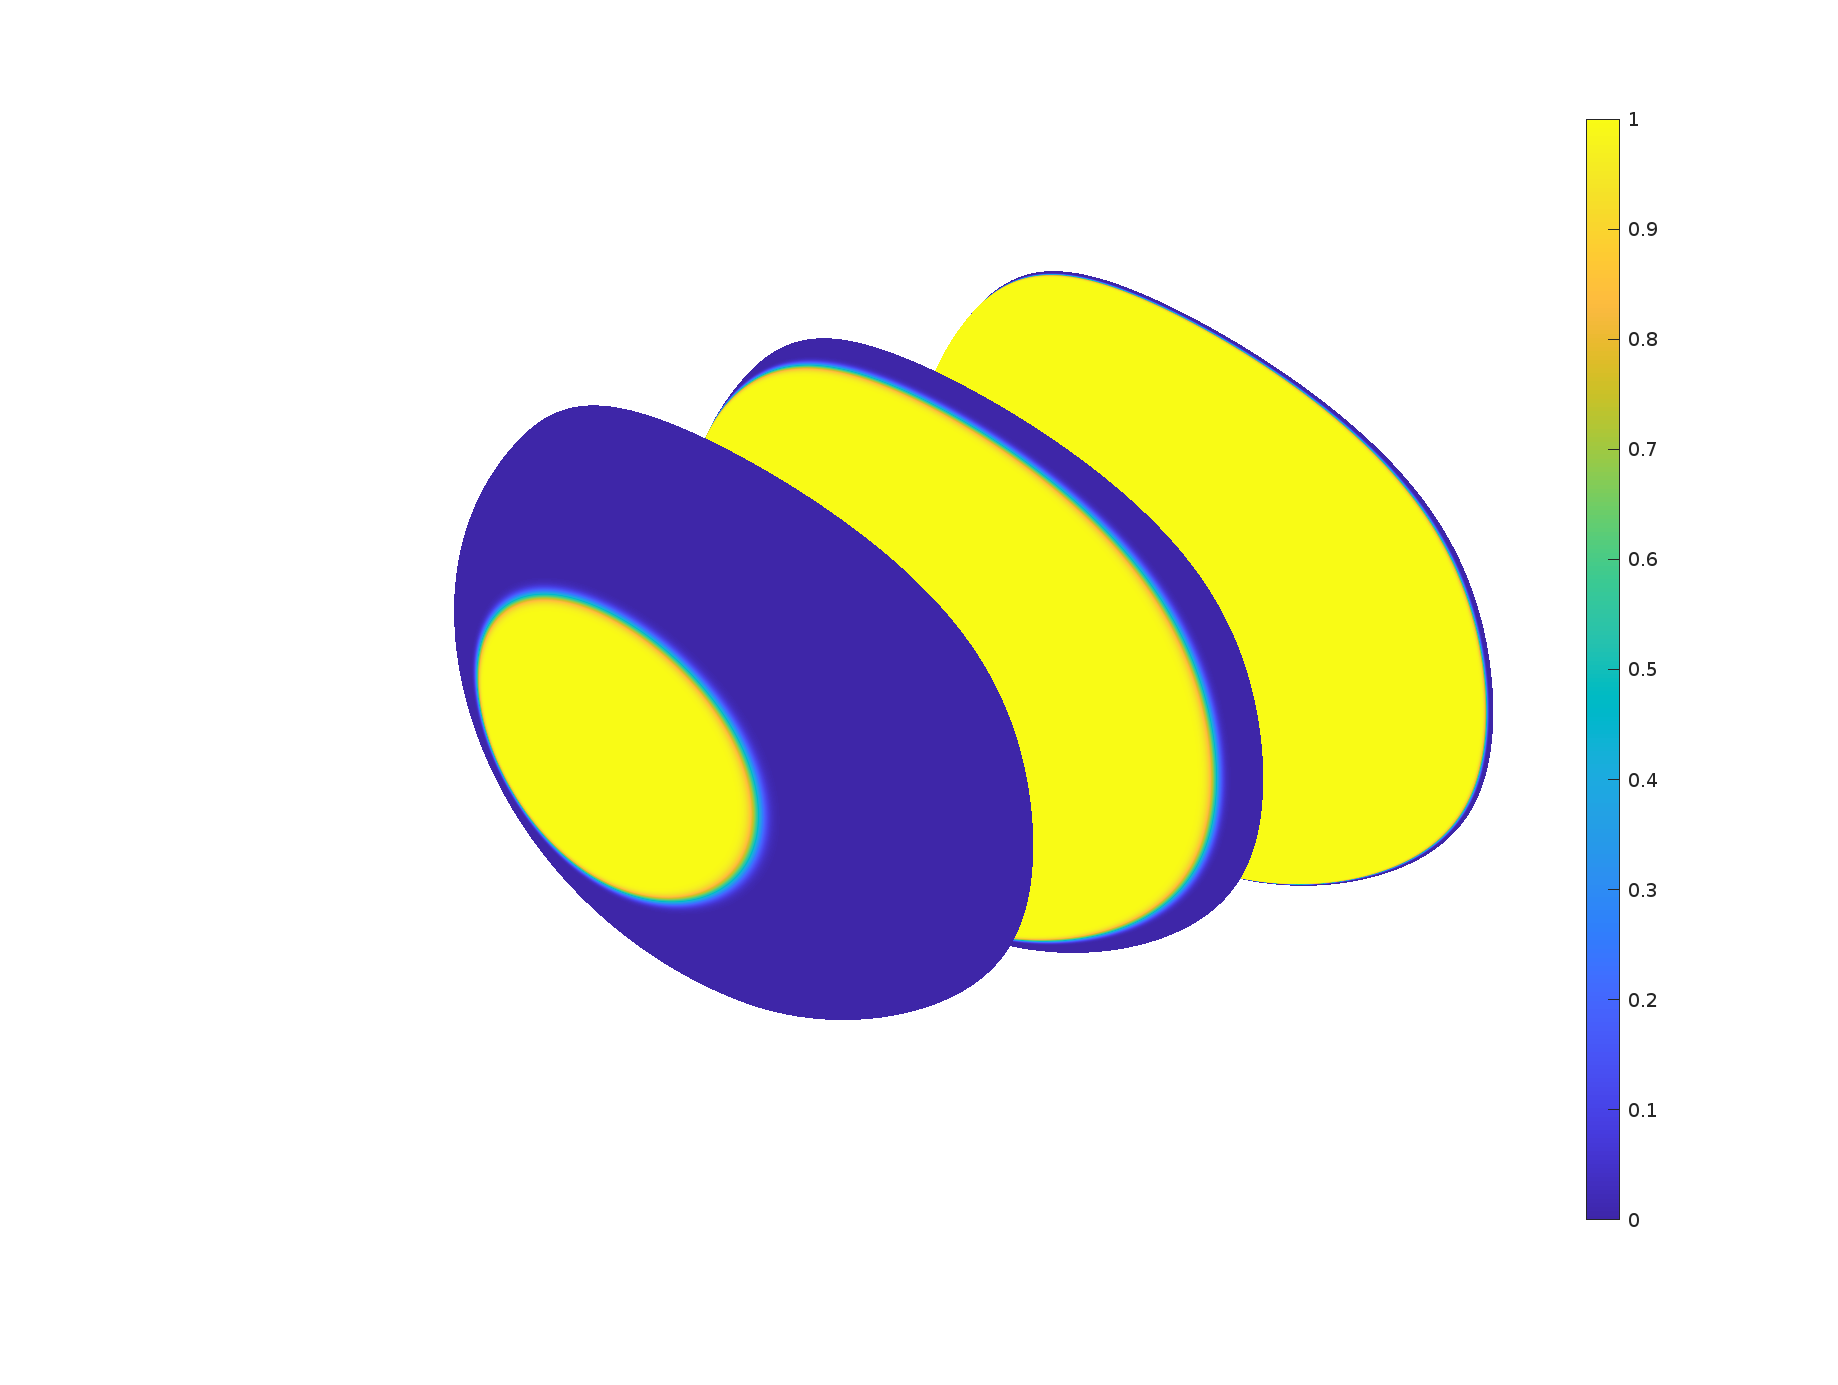
\includegraphics[scale = 0.3]{Images/Exponents.eps}};
                    \node at (0, -2) {\({p=1}\)};
                    \node at (1.2, -1.6) {\({p=4}\)};
                    \node at (2.4, -1.2) {\({p=7}\)};
                \end{tikzpicture}
                \caption{Auswirkung des \({p}\) der \({F_p}\) auf die resultierenden Karten der Konstruktion \ref{sec:part_one:good_atlas:force_cover:new_atlas}.}
                \label{fig:part_one:good_atlas:force_cover_new_atlas:ex0}
            \end{figure}
        
    \subsection{Existenz eines guten Atlas}
    \label{sec:part_one:good_atlas:exists}
        Wir wenden uns nun der Existenz eines guten Atlas zu. Der Beweis beruht grundlegend auf der echt aufsteigenden kompakten \"Uberdeckung aus Lemma \ref{lem:top_man:rel_comp_cover}. Folgende Beweisidee ist in Abbildung \ref{fig:part_one:good_atlas:exist:ex0} dargestellt. 
        Wir wenden uns nun der Existenz eines guten Atlas zu. Der Beweis beruht grundlegend auf der echt aufsteigenden kompakten \"Uberdeckung aus Lemma \ref{lem:top_man:rel_comp_cover}, und verl\"auft \"ahnlich zu dem der Parakompaktheit. Folgende Beweisidee ist in Abbildung \ref{fig:part_one:good_atlas:exist:ex0} dargestellt. 
        \begin{theorem}[Existenz eines guten Atlas]
            \label{thm:part_one:good_atlas:exists:exists}
            Eine differenzierbare Mannigfaltigkeit \({\mathcal{M}}\) besitzt zu jeder beliebigen offenen \"Uberdeckung \({\mathfrak{U}}\) einen untergeordneten guten Atlas.
        \end{theorem}
        \begin{proof}
            Da \({\mathcal{M}}\) lokalkompakt und zweitabz\"ahlbar ist, existiert nach Lemma \ref{lem:top_man:comp_asc_cover} eine echt aufsteigende kompakte \"Uberdeckung \({A_k}\). Seien
            \[S_k^1:=A_k\setminus\mathring{A}_{k-1}\quad\text{und}\quad S_k^2:=A_{k+1}\setminus\mathring{A}_{k-2}\]
            erneut kompakt. Weiter gibt es f\"ur jedes \({\mathbf{y}\in S_k^1}\) eine Karte \({\alpha_{i_{\mathbf{y}}}\colon V_{i_{\mathbf{y}}}\to U_{i_{\mathbf{y}}}}\) mit \({U_{i_{\mathbf{y}}}\subseteq S_k^2}\), sei also \({\mathbf{x}=\alpha^{-1}_{i_{\mathbf{y}}}(\mathbf{y})}\). Da \({\alpha_{i_{\mathbf{y}}}}\) stetig ist, ist das Urbild von \({U_{i_{\mathbf{y}}}\cap\mathring{S}_k^2}\) unter \({\alpha_{i_{\mathbf{y}}}}\) offen (und nicht leer), und wir k\"onnen einen Radius \({\epsilon_{\mathbf{y}}}\) finden, sodass
            \begin{equation}
                \label{eq:part_one:good_atlas:abstr_con:0}
                \Delta_{\mathbf{y}}:=B_{\frac{\epsilon_{\mathbf{y}}}{3}}\left(\mathbf{x}\right)\subset B_{\epsilon_{\mathbf{y}}}\left(\mathbf{x}\right)\subseteq\alpha_{i_{\mathbf{y}}}^{-1}\left(U_{i_{\mathbf{y}}}\cap\mathring{S}_k^2\right)\,.
            \end{equation}
            Die \({\left(\alpha_{i_{\mathbf{y}}}\left(\Delta_{\mathbf{y}}\right)\right)_{\mathbf{y}\in S_k^1}}\) bilden nun offenbar eine offene \"Uberdeckung von \({S_k^1}\). Da \({S_k^1}\) kompakt ist, besitzt diese eine endliche Teil\"uberdeckung, es existiert also eine endliche Teilmenge \({S^{\prime}_k\subset S_k^1}\), sodass
            \begin{equation}
            \label{aaarar}
                S_k^1\subset\bigcup_{\mathbf{z}\in S_k^{\prime}}\alpha_{i_{\mathbf{z}}}\left(\Delta_{\mathbf{z}}\right)\mathop{\subset}^{\eqref{eq:part_one:good_atlas:abstr_con:0}}\mathring{S}_k^2\cap\bigcup_{\mathbf{z}\in S_k^{\prime}}U_{i_{\mathbf{z}}}\subseteq\mathring{S}_k^2
            \end{equation}
            gilt. Wir definieren
            \[\beta_{\mathbf{y}}\colon B_1\to\alpha_{i_{\mathbf{y}}}\left(B_{\epsilon_{\mathbf{y}}}\right),\,\mathbf{z}\mapsto\alpha_{i_{\mathbf{y}}}\left(\epsilon_{\mathbf{y}}\cdot\mathbf{z}\right)\hspace{1.5cm}\forall\mathbf{y}\in S_k^{\prime}\,,\]
            und erhalten letztenendes mit
            \[\left\{\beta_{\mathbf{y}}\colon B_1\to\alpha_{i_{\mathbf{y}}}\left(B_{\epsilon_{\mathbf{y}}}\right)\big|\,\forall\mathbf{y}\in S_k^{\prime}\colon\forall k\in\mathbb{N}\right\}\]
            den gesuchten abz\"ahlbaren Atlas. Die lokale Endlichkeit folgt dabei aus \ref{aaarar}.
        \end{proof}
    
        \begin{figure}
            \centering
            \fbox{
            \small
            \begin{tikzpicture}[scale = 1.4]
    
                \draw   (165:4) node at +(-1, 1) (c1) {}
                        (165:4) node at +(1, -1) (c2) {}
                        (130:4) node at +(1, 0) (c3) {};
                        
                \begin{scope}[line width = 0pt]
                
                    \path [pattern = north east lines] 
                        (0, 4) arc (90:180:4) -- (-3, 0) arc (180:90:3) -- cycle
                        (0, 2) arc (90:180:2) -- (-1, 0) arc (180:90:1) -- cycle;
                        
                    \path [pattern = north west lines] 
                        (0, 3) arc (90:180:3) -- (-2, 0) arc (180:90:2) -- cycle;
                    
                    \fill [white]
                        (130:4) .. controls ++(-1, 0) and (c1) .. (165:4)
                        .. controls (c2) and (-0.5, 1) .. (-1.5, 1.5)
                        .. controls (-2.5, 2) and (c3) .. (130:4) -- cycle;
           
                \end{scope}
    
                \draw
                    \foreach\r in {1,2,3,4}{ (0, \r) arc (90:180:\r) }
                    
                    (-3, 0.8) .. controls (-2.2, 0.4) and (-2, 0.8) .. (-2.4, 1.2)
                    .. controls (-2.8, 1.6) and (-2, 2.8) .. (-2.8, 2.4)
                    .. controls (-3.6, 2) and (-3.8, 1.2) .. (-3, 0.8)% node [pos = 0, above, sloped] {\({U_{i_{\mathbf{x}}}}\)}
                    
                    (-2.7, 0.8) .. controls (-2.5, 0.7) and (-2.4, 0.8) .. (-2.5, 1.1)
                    .. controls (-2.6, 1.4) and (-2.5, 2.3) .. (-3, 1.8)% node [pos = 0.9, above, sloped] {\({U_{i_{\mathbf{x}}}}\)}
                    .. controls (-3.5, 1.3) and (-2.9, 0.9) .. (-2.7, 0.8)
                    
                    (1, 1.5) .. controls (1.4, 1.6) and (1.6, 2.8) .. (2.2, 2.6)
                    
                    (-2.7, 1) node {\tiny\textbullet}
                    (2, 1) node {\tiny\textbullet}
                    ++(2/9, 0) arc (0:360:2/9) node [pos = 0.125, sloped, above] {\({\Delta_{\mathbf{x}}}\)}
                    ++(4/9, 0) arc (0:360:2/3) node [pos = 0.125, sloped, above] {\({B_{\epsilon_{\mathbf{x}}}}\)}
                    
                    (2, 4) node {\({\mathbb{R}^n}\)}
                    (-2.7, 4) node {\({\mathcal{M}}\)};
                
                \begin{scope}[line width = 1pt]
                    \draw [dashed, line width = 1pt] 
                        (130:4) .. controls ++(-1, 0) and (c1) .. (165:4) node [pos = 0.3, above, sloped] {\({U_{i_{\mathbf{x}}}}\)}
                        (2.2, 2.6) .. controls (1.2, 3.4) and (1, 2.5) .. (1, 1.5);
        
                    \draw (1, 1.5) .. controls (1, 0.5) and (1.5, 0) .. (2.6, 0.4)
                        .. controls (3.7, 0.8) and (3.2, 1.8) .. (2.2, 2.6) node [pos = 0.75, sloped, above] {\({V_{i_{\mathbf{x}}}}\)}
                        (165:4) .. controls (c2) and (-0.5, 1) .. (-1.5, 1.5)
                        .. controls (-2.5, 2) and (c3) .. (130:4);
                \end{scope}
    
                        
                \draw [decorate, decoration = {calligraphic brace, raise=3pt, amplitude = 5pt}] (-2, 0) -- node [below = 5pt] {\({S_k^1}\)} (-3, 0);
                \draw [decorate, decoration = {calligraphic brace, raise=18pt, amplitude = 10pt}] (-1, 0) -- node [below = 25pt] {\({S_k^2}\)} (-4, 0);
    
                \draw [->] (1.75, 1.25) [bend right] to node [pos = 0.3, above] {\({\alpha_{i_{\mathbf{x}}}}\)} (-2.4, 1.25);
            \end{tikzpicture}
            }
            \caption{Konstruktion eines guten Atlas}
            \label{fig:part_one:good_atlas:exist:ex0}
        \end{figure}

\section{Konstruktion einer Zerlegung der Eins}
\label{sec:part_one:constr_one}
    Ein gegebener guter Atlas erm\"oglicht uns nun, eine Zerlegung der Eins zu konstruieren. Sei hierzu zun\"achst
    \[\lambda\colon\mathbb{R}\to[0,1[,\,t\mapsto\begin{cases}
        e^{-\frac{1}{t^2}} & t>0\\
        0 & \text{sonst}
    \end{cases}\,.\]
    Man sieht, dass die Ableitung dieser Funktion 
    \[\frac{\text{d}^n\lambda}{\text{d}^nt}=r_n(t)\lambda(t)\]
    mit einer rationalen Funktion \({r_n}\) ist. Wir zeigen mittels Induktion, dass \({\lambda}\) glatt ist. Sowohl der Induktionsanfang als auch der Induktionsschritt folgen aus
    \[\lambda^{(n)}(0)=\lim_{\genfrac{}{}{0pt}{}{h\to0}{h\not=0}}\frac{\lambda^{(n-1)}(h)-\lambda^{(n-1)}(0)}{h}=\lim_{\genfrac{}{}{0pt}{}{h\to0}{h\not=0}}\frac{r_{n-1}(h)e^{-\frac{1}{h^2}}-0}{h}=0\,.\]
    Der Tr\"ager von \({\lambda}\) ist \({\text{supp}(\lambda)=\mathbb{R}_{\geq0}}\). Wir setzen nun
    \[\phi\colon\mathbb{R}\to[0,1],\,t\mapsto\frac{\lambda(t)}{\lambda(t)+\lambda(1-t)}\,,\]
    sodass wir eine differenzierbare Funktion erhalten, die f\"ur \({t\leq0}\) verschwindet und f\"ur \({t\geq1}\) gleich eins ist. Sei weiter
    \[\psi\colon\mathbb{R}^n\to[0,1],\,\mathbf{x}\mapsto1-\phi\left(3\norm{\mathbf{x}}-1\right)\,,\]
    eine Funktion mit Tr\"ager \({\overline{B_{\nicefrac{2}{3}}}}\). Wir definieren f\"ur \({i\in\Lambda}\) die Funktionen
    \[\omega_i\colon\mathcal{M}\to[0,1],\,\mathbf{x}\mapsto\begin{cases}
        \left(\psi\circ\alpha_i^{-1}\right)(\mathbf{x}) & \mathbf{x}\in\alpha_i\left(B_{\nicefrac{2}{3}}(0)\right)\\
        0 & \text{sonst}
    \end{cases}\,,\]
    die aufgrund der lokalen Endlichkeit summierbar sind - f\"ur jedes \({\mathbf{x}\in\mathcal{M}}\) sind lediglich endlich viele \({\omega_i(\mathbf{x})\not=0}\). Da die \({\alpha_i\left(B_{\nicefrac{2}{3}}(0)\right)}\) immer noch eine \"Uberdeckung von \({\mathcal{M}}\) bilden, ist die Summe au\ss erdem \"uberall ungleich null. Wir erhalten final die nun wohldefinierten
    \[\theta_i:=\frac{\omega_i}{\sum_{j\in\Lambda}\omega_j}\,,\]
    die wegen
    \[\sum_{i\in\Lambda}\theta_i=\frac{\sum_{i\in\Lambda}\omega_i}{\sum_{j\in\Lambda}\omega_j}=1\]
    eine Teilung der Eins darstellen. Da der Nenner stets mindestens so gro\ss{} wie der Z\"ahler ist, ist zudem \({0<\theta_i\leq 1}\).
    
\section{Beispiel Teilung der Eins}
\label{sec:part_one:ex0}
    Bezeiche im Folgenden stets
    \[E_{a,b}=\left\{\mathbf{x}\in\mathbb{R}^2\colon\sqrt{\left(\frac{x_1}{a}\right)^2+\left(\frac{x_2}{b}\right)^2}\leq1\right\}\]
    die Ellipse mit Radien \({a}\) und \({b}\).
    Wir betrachten die Nullstellenmenge des Gleichungssystems
    \begin{align}
        \cos(x)+\cos(y)-z^2&=1
    \end{align}
    im \({\mathbb{R}^3}\). Sei \({\mathcal{M}}\) die Zusammenhangskomponente nahe des Ursprungs. L\"osen wir jeweils in eine Richtung auf, erhalten wir naiv sechs Karten. Mit den Bezeichnungen \({U=\{0<\cos(x)-y^2\leq1\}}\) und \({V=\{1<\cos(x)+\cos(y)\leq2\}}\) ergeben sich explizit
    \[\gamma_{1,2}\colon U\to\mathcal{M},\mathbf{x}\mapsto\left(\pm\arccos\left(\cos(x)-y^2-1\right),x,y\right)^T\]
    \[\gamma_{3,4}\colon U\to\mathcal{M},\mathbf{x}\mapsto\left(x,\pm\arccos(\cos(x)-y^2-1),y\right)^T\]
    \[\gamma_{5,6}\colon V\to\mathcal{M},\mathbf{x}\mapsto\left(x,y,\pm\sqrt{\cos(x)+\cos(y)-1}\right)^T\,.\]
    Obgleich es sicher scheint, dass \({B_1}\), \({U}\) und \({V}\) zueinander diffeomorph sind, ist es nicht einfach explizite Diffeomorphismen anzugeben. Anstelle dessen betrachten wir die hinreichend gro\ss en einfacheren Teilmengen \({E_{\nicefrac{3}{2},\nicefrac{9}{10}}\subset U}\) und \({B_{\nicefrac{4}{3}}\subset V}\) und die induzierten Karten
    \[\beta_i:=\begin{cases}
        \gamma_i\mathrel{|}_{E_{\nicefrac{3}{2},\nicefrac{9}{10}}} & 1\leq i\leq4\\
        \gamma_i\mathrel{|}_{B_{\nicefrac{4}{3}}} & \text{sonst}
    \end{cases}\,,\]
   die immer noch einen Atlas von \({\mathcal{M}}\) bilden (ohne Beweis). Da der Atlas endlich ist, k\"onnen wir Wie in Sektion \ref{sec:part_one:good_atlas:force_cover} beschrieben erhalten wir aus den \({\beta_i}\) nun einen Atlas \({\{\alpha_i\to M\}}\), der aufgrund der Endlichkeit des vorherigen Atlas auch gut ist. Dieser, und die von ihm implizierte Teilfunktionen der Zerlegung der eins sind in Abbildung \ref{fig:part_one:good_atlas:exist:ex0} dargestellt.
    
    \begin{figure}
        \centering
        \begin{subfigure}{0.49\textwidth}
            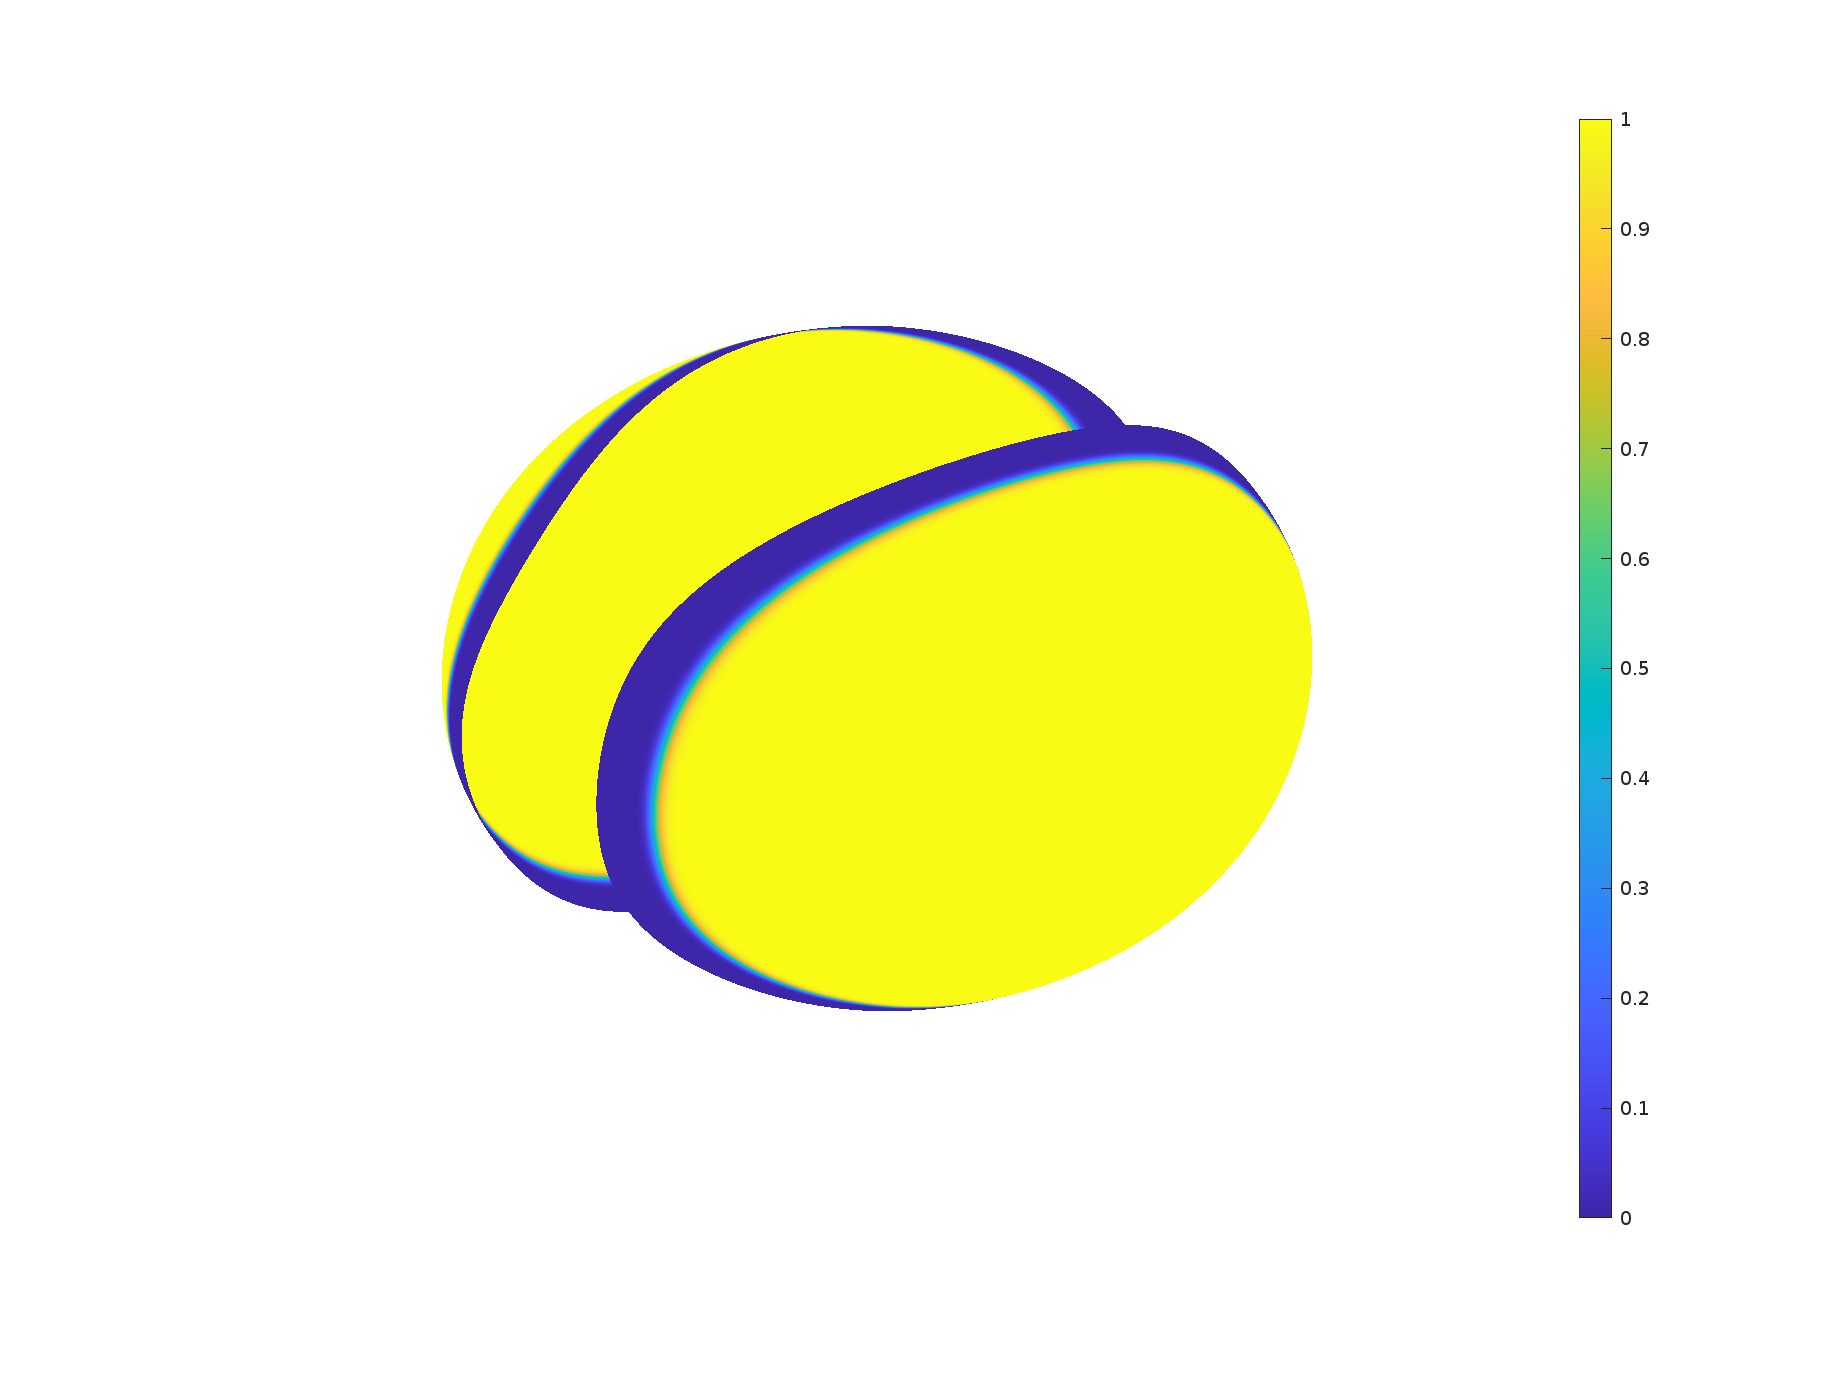
\includegraphics[scale = 0.2]{Images/PoO_01.eps}
            \caption{Die Karten \({\alpha_1}\) und \({\alpha_2}\).}
        \end{subfigure}
        \begin{subfigure}{0.49\textwidth}
            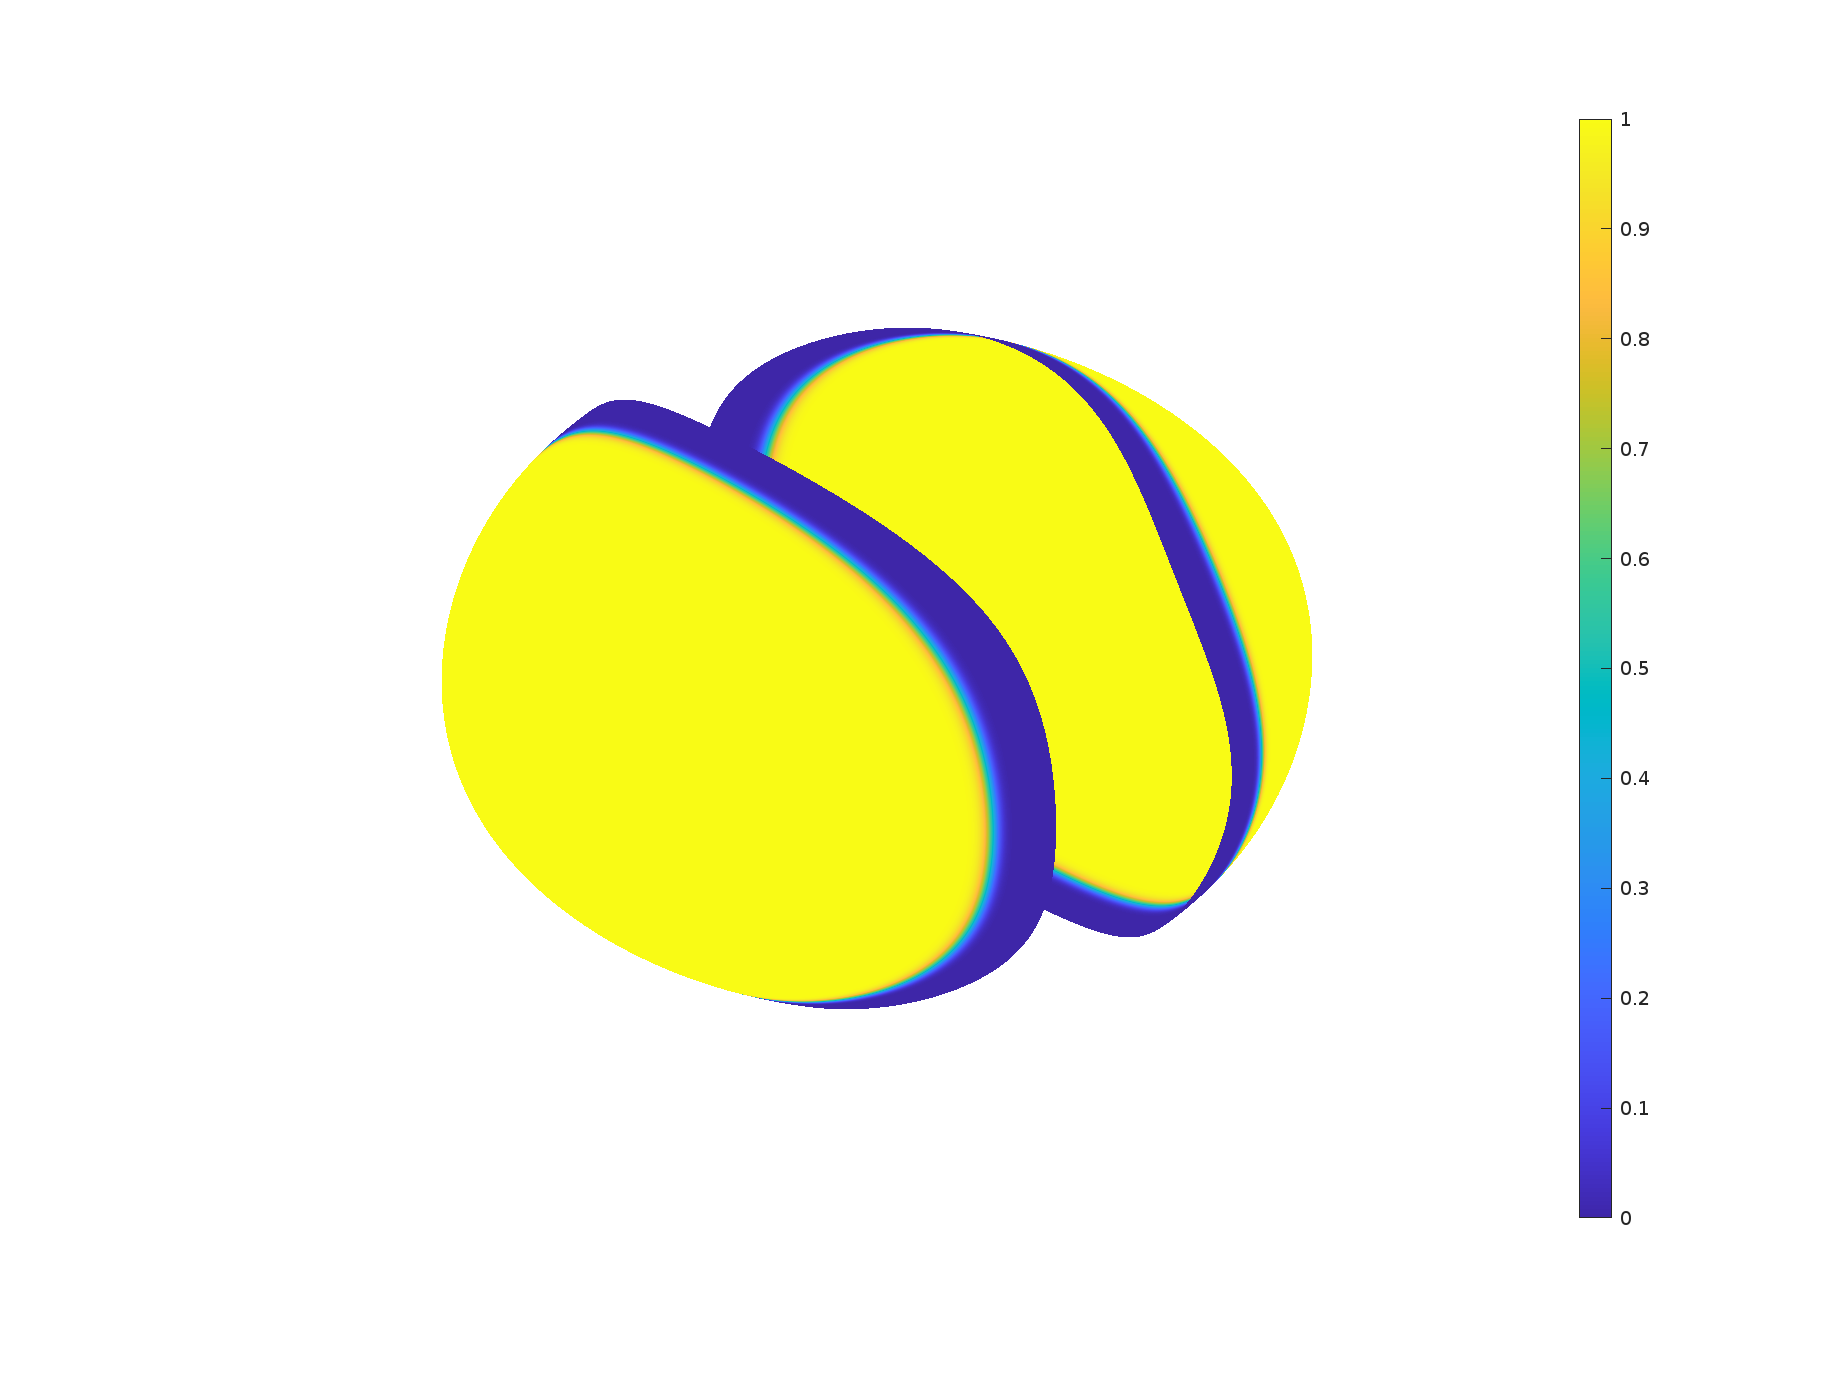
\includegraphics[scale = 0.2]{Images/PoO_02.eps}
            \caption{Die Karten \({\alpha_3}\) und \({\alpha_4}\).}
        \end{subfigure}
        \begin{subfigure}{0.49\textwidth}
            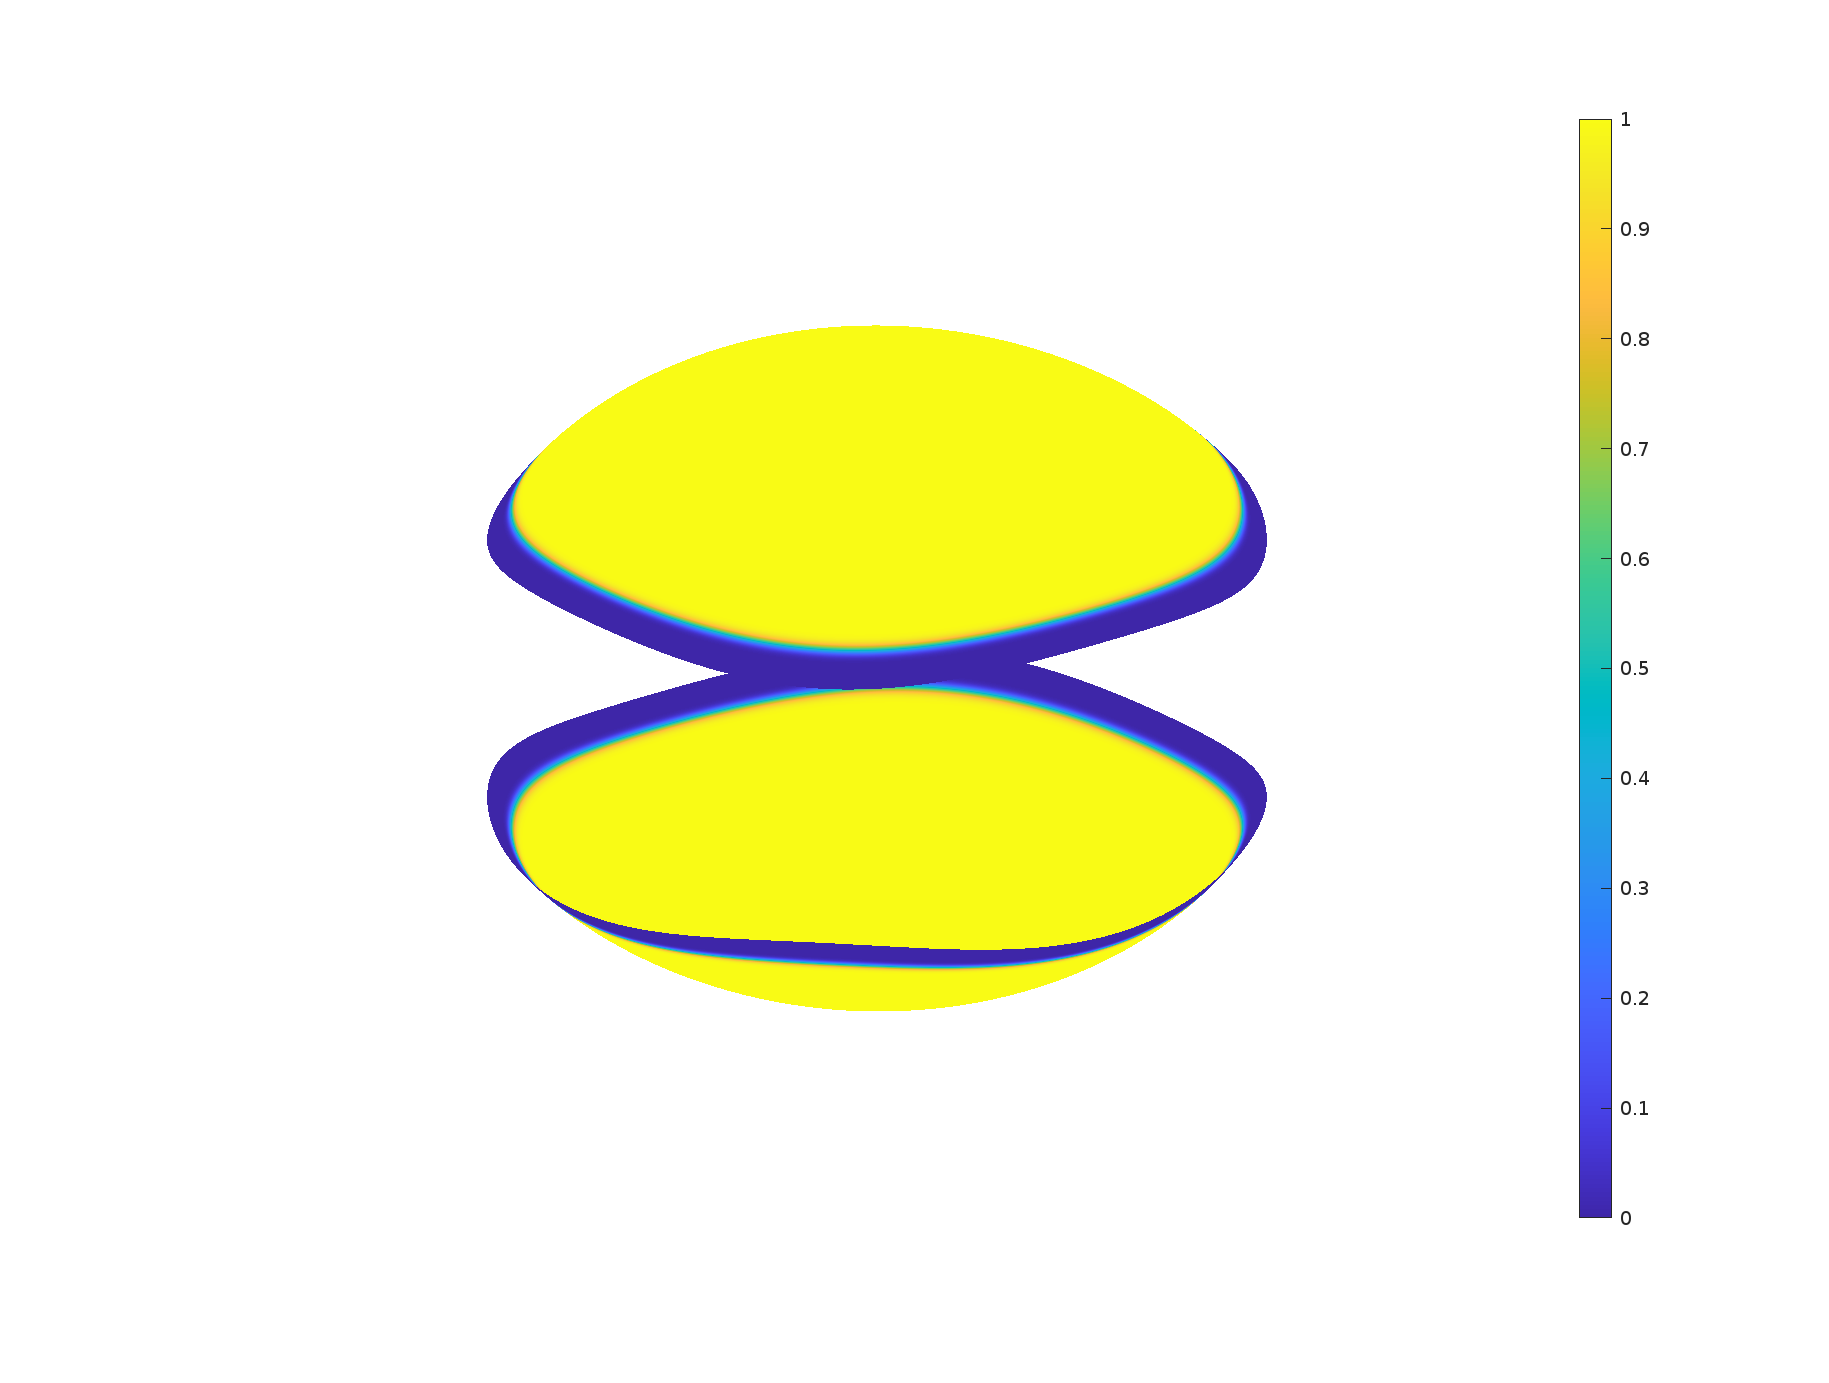
\includegraphics[scale = 0.2]{Images/PoO_03.eps}
            \caption{Die Karten \({\alpha_5}\) und \({\alpha_6}\).}
        \end{subfigure}
        \begin{subfigure}{0.49\textwidth}
            
\includegraphics[scale = 0.2]{Images/PoO_04.eps}
            \caption{Die Summe der \({\theta_i}\) auf \({M}\).}
            \label{fig:part_one:ex0:ex0:ex0}
        \end{subfigure}
        \caption{Die sechs Karten von \({\mathcal{M}}\) f\"ur \({p=4}\). Die Farbe beschreibt die Magnit\"ude der zugeh\"origen \({\theta_i}\).}
        \label{fig:part_one:ex0:ex0}
    \end{figure}

    \subsection{Visualisierung}
        Um eine gut konditionierte Parametrisierung von \({\mathcal{M}}\) (Abbildung \ref{fig:part_one:ex0:ex0:ex0}) zu erhalten wurde eine Einheitssph\"are parametrisiert (Kugelkoordinaten) und f\"ur jeden Punkt \({(x,y,z)^T\in S^2}\) das Newton-Verfahren auf die Funktion
        \[f(r)=\cos(rx)+\cos(ry)-(rz)^2-1\]
        angewandt, also einige Iterationen 
        \[r_{n+1}=r_n+\frac{\cos(r_nx)+\cos(r_ny)-(r_nz)^2-1}{x\sin(r_nx)+y\sin(r_ny)+2z^2r_n}\]
        mit \({r_0=\frac{\pi}{4}}\) berechnet. Da dieses gegen eine Nullstelle von \({f}\) konvergiert, konvergiert \({r_n\cdot(x,y,z)^T}\) gegen einen Punkt in \({\{\cos(x)+\cos(y)-z^2=1\}}\), also auch wahrscheinlich gegen einen Punkt in \({M}\). Auch wenn das Ergebnis aus der Perspektive wie eine Kugel aussieht, ist dies nicht der Fall. Die Visualisierung erfolgte in Matlab R2023a.
        
    \chapter{Der Immersionssatz}
        Im folgenden Abschnitt wollen wir den Immersionssatz beweisen. Dieser garantiert, dass eine differenzierbare Funktion \({\mathcal{M}\to\mathbb{R}^n}\) f\"ur hinreichend gro\ss es \({n}\) beliebig gut durch eine Immersion approximieren l\"asst. Dieses Ergebnis wird sp\"ater noch weiter verfeinert werden.

Sei \({\norm{\mathrel{\cdot}}_1}\) die Summennorm auf dem \({\mathbb{R}^n}\), \({U\subset\mathbb{R}^m}\) offen, und \({H\in\mathcal{C}\left(U,\mathbb{R}^n\right)}\). Im Folgenden wollen wir den Raum \({\mathcal{C}\left(U,\mathbb{R}^n\right)}\) mit einer Topologie versehen. Sei hierzu
\[\norm{H}_C:=\max_{p\in C}\left(\norm{H(p)}_1\right)\]
die Supremumsnorm auf der kompakten Menge \({C\subset U}\), und weiter
\[\norm{H}:=\norm{H}_C+\sum_{j=1}^m\norm{\frac{\partial H}{\partial x_j}}_C\,.\]
Dies definiert keine Norm auf \({\mathcal{C}\left(U,\mathbb{R}^n\right)}\), da \({H}\) lediglich auf \({C}\) betrachtet wird, nicht jedoch \({U\setminus C}\). Demnach folgt aus \({\norm{H}=0}\) nicht dringend \({H=0}\). Dennoch induziert diese Seminorm eine Topologie, welche wir im Weiteren betrachten wollen. Es sei angemerkt, dass bei der Definition dieser Seminorm lediglich die erste Ableitung in das Ergebnis einflie\ss t. Zwar ist es m\"oglich dies zu verallgemeinern indem alle Supremumsnormen partieller Ableitungen vom Grad \({\leq k}\) aufsummiert werden, jedoch ist dies f\"ur den schwachen Einbettungssatz nicht vonn\"oten - Lediglich die erste Ableitung muss sich einigerma\ss en friedlich verhalten. 

\begin{theorem}[Die Menge der regul\"aren Funktionen ist offen]
\label{thm:imm_thm:reg_open}
    Sei \({m\leq n}\), \({U\subset\mathbb{R}^m}\) offen und \({K\subset U}\) kompakt, so ist die Menge der in \({K}\) regul\"aren Funktionen offen in \({\mathcal{C}\left(U,\mathbb{R}^n\right)}\).
\end{theorem}
\begin{proof}
    Sei \({\mathbf{x}\in\mathbb{R}^m}\). Unter der zuvor definierten Seminorm ist die Abbildung
    \[\Phi\colon C^k\left(U,\mathbb{R}^n\right)\to\mathbb{R}^{n\times m},\,F\mapsto J_{\mathbf{x}}F\]
    stetig. Sei hierzu der \({\mathbb{R}^{n\times m}}\) mit der Spaltensummennorm versehen. Dies mag beliebig wirken, ist jedoch dadurch gerechtfertigt, dass alle Normen auf einem endlichdimensionalen reellen Vektorraum \"aquivalent sind. Sei weiter \({0<\delta\leq\epsilon}\) und \({\norm{F-G}<\delta}\). Es folgt
    \begin{align*}
        \norm{J_{\mathbf{x}}(F-G)}_1&=\max_{1\leq j\leq m}\norm{\frac{\partial(F-G)}{\partial x_j}(\mathbf{x})}_1\\
        &\leq\max_{1\leq j\leq m}\norm{\frac{\partial(F-G)}{\partial x_j}}_K\\
        &<\norm{F-G}<\delta<\epsilon
    \end{align*}
    und aus dem \({\epsilon}\)-\({\delta}\)-Kriterium die Stetigkeit der Abbildung \({H\mapsto J_{\mathbf{x}}H}\). Dieses gilt weiterhin, da die Topologie mittels der Seminorm definiert wurde. Wir betrachten weiter die stetige Abbildung
    \[\Psi\colon\mathbb{R}^{n\times m}\to\mathbb{R},\,A\mapsto\sum_{\genfrac{}{}{0pt}{}{B\,\text{ist}\,m\times m}{\genfrac{}{}{0pt}{}{\text{Untermatrix}}{\text{von}\,A}}}\abs{\det\left(B\right)}\,.\]
    Wenn \({A}\) den Rang \({m}\) besitzt, so existiert bekannterma\ss en eine invertierbare \({m\times m}\) Untermatrix vom \({A}\). Somit gilt \({\Psi(A)\not=0}\). Aufgrund der Stetigkeit ist nun
    \[\Psi^{-1}\left(\mathbb{R}\setminus\{0\}\right)=\left\{B\in\mathbb{R}^{n\times m}\colon\text{rang}(B)=m\right\}=:B^{\prime}\]
    offen, sodass auch 
    \[\Phi^{-1}\left(B^{\prime}\right)=\left\{F\in\mathcal{C}^k\left(U,\mathbb{R}^n\right)\colon\text{rang}(F)=m\right\}\]
    offen ist.
\end{proof}

Der Beweis des Faktes, dass die Menge der Matrizen mit vollem Rang offen ist, wurde \cite{test} entnommen.

\begin{theorem}
\label{thm:imm_thm:reg_dense}
    Sei \({U\subset\mathbb{R}^n}\) offen und \({K\subset U}\) kompakt, so ist die Menge der in \({K}\) regul\"aren Funktionen dicht in \({\mathcal{C}\left(U,\mathbb{R}^n\right)}\), wenn \({n\geq2m}\).
\end{theorem}
\begin{proof}
    Sei \({F\in\mathcal{C}\left(U,\mathbb{R}^n\right)}\) und \({\epsilon>0}\). Wir konstruieren f\"ur \({1\leq k\leq m}\) Funktionen \({G_k\colon U\to\mathbb{R}^n}\), sodass die ersten \({k}\) Ableitungsvektoren \({\partial G_k/\partial x_j}\) voneinander linear unabh\"angig sind. Per Konstruktion ist dann \({G:=G_m}\) regul\"ar. Sei \({G_0:=F}\), \({G_{k-1}}\) bereits konstruiert und 
    \begin{equation}
        \label{eq:imm_thm:reg_dense:1}
        c:=\max_{\genfrac{}{}{0pt}{}{\mathbf{x}\in C}{1\leq j\leq m}}\abs{x_j}\,.
    \end{equation}
    Wir betrachten die Hilfsfunktion
    \[\Phi_k\colon\mathbb{R}^{k-1}\times U\to\mathbb{R}^n,\binom{\lambda}{\mathbf{x}}\mapsto\sum_{j=1}^{k-1}\lambda_j\frac{\partial G_{k-1}}{\partial x_j}(\mathbf{x})-\frac{\partial F}{\partial x_k}(\mathbf{x})\,,\]
    dann finden wir mithilfe des Satzes von Sard aufgrund von 
    \[\text{dim}(\mathbb{R}^k\times U)=k+m-1<2m\leq n\]
    ein \({\mathbf{a}_k\in\mathbb{R}^n\setminus\text{Bild}(\Phi_k)}\), sodass
    \begin{equation}
        \label{eq:imm_thm:reg_dense:2}
        \norm{\mathbf{a}_k}<\frac{\epsilon}{m\left(c+1\right)}\,.
    \end{equation}
    Wir setzen 
    \[G_k:=G_{k-1}+x_k\cdot\mathbf{a}_k\,,\]
    dann sind
    \[\frac{\partial G_k}{\partial x_i}(\mathbf{x})=\frac{\partial G_{k-1}}{\partial x_i}(\mathbf{x})\quad\text{f\"ur}\quad1\leq i<k\quad\text{und}\quad\frac{\partial G_k}{\partial x_k}(\mathbf{x})=\frac{\partial F}{\partial x_k}(\mathbf{x})+\mathbf{a}_k\,.\]
    Die ersten \({k}\) dieser Vektoren sind nun f\"ur alle \({\mathbf{x}\in U}\) linear unabh\"angig, da sonst
    \[\sum_{j=1}^{k-1}\lambda_j\frac{\partial G_k}{\partial x_j}(\mathbf{x})=\frac{\partial G_k}{\partial x_k}(\mathbf{x})\quad\Leftrightarrow\quad\sum_{j=1}^{k-1}\lambda_j\frac{\partial G_{k-1}}{\partial x_j}(\mathbf{x})-\frac{\partial F}{\partial x_k}(\mathbf{x})=\mathbf{a}_k\]
    ein Widerspruch gegen die Definition von \({\mathbf{a}_k}\) w\"are. Letztlich sei \({G:=G_m}\), so ergibt sich die Absch\"atzung
    \newpage
    \begin{align*}
        \norm{G-F}&=\norm{G_m-G_0}=\norm{\sum_{k=1}^mG_k-G_{k-1}}\\
        &\mathop{\leq}^{\Delta}\sum_{k=1}^m\norm{G_k-G_{k-1}}\mathop{=}^{\text{Def.}}\sum_{k=1}^m\norm{x_k\cdot\mathbf{a}_k}\\
        &=\sum_{k=1}^m\left(\max_{\mathbf{x}\in C}\abs{x_k}\norm{\mathbf{a}_k}_1+\norm{\mathbf{a}_k}_1\right)\mathop{\leq}^{\eqref{eq:imm_thm:reg_dense:1}}\sum_{k=1}^m\norm{\mathbf{a}_k}\left(c+1\right)\\
        &\mathop{<}^{\eqref{eq:imm_thm:reg_dense:2}}\frac{1+c}{1+c}\cdot\epsilon\sum_{k=1}^m\frac{1}{m}=\epsilon\,.
    \end{align*}
\end{proof}

\begin{theorem}[Whitneyscher Immersionssatz]
\label{thm:imm_thm:imm_thm}
    Sei \({n\geq2m}\), \({\mathcal{M}^m}\) eine differenzierbare Mannigfaltigkeit sowie \({\delta>0}\) und \({F\colon\mathcal{M}\to\mathbb{R}^n}\) regul\"ar in der abgeschlossenen Menge \({A\subseteq\mathcal{M}}\). Dann existiert eine Immersion \({G\colon\mathcal{M}\to\mathbb{R}^n}\) derart, dass \({G|_A=F|_A}\) und f\"ur alle \({p\in\mathcal{M}}\) die Absch\"atzung \({\norm{F(p)-G(p)}<\delta}\) gilt.
\end{theorem}
\begin{proof}
    Da der Rang von \({F}\) lokal nicht fallen kann, existiert eine offene Umgebung \({U\subseteq\mathcal{M}}\) von \({A}\), auf der \({F}\) weiterhin vollen Rang besitzt. Wir betrachten die offene \"Uberdeckung \({\{U,\mathcal{M}\setminus A\}}\) von \({\mathcal{M}}\) und w\"ahlen mithilfe von Satz \ref{thm:part_one:good_atlas:exists:exists} einen untergeordneten guten Atlas \({\left\{\alpha_k\colon B_1\to V_k\right\}}\), sowie eine zugeh\"orige Zerlegung der Eins \({\theta_k\colon\mathcal{M}\to[0,1]}\) gem\"a\ss{} Sektion \ref{sec:part_one:constr_one}.
    \[K:=\overline{B_{\nicefrac{2}{3}}}\quad,\quad U_k:=\alpha_k\left(B_{\nicefrac{1}{3}}\right)\quad\text{sowie}\quad W_k:=\alpha_k\left(B_{\nicefrac{2}{3}}\right)\,.\]
    %F\"ur folgende Absch\"atzungen ben\"otigen wir noch 
    %\[\epsilon_k:=2^{-k}\inf\left\{\delta\left(W_k\right)\right\}\]
    Wir konstruieren nun f\"ur \({k\geq1}\) eine Folge von Funktionen \({G_k}\) mit folgenden Eigenschaften
    \begin{align}
        \label{eq:imm_thm:imm_thm:0}
        G_k(p)=G_{k-1}(p)\qquad&\forall p\in\mathcal{M}\setminus W_k\\
        \label{eq:imm_thm:imm_thm:1}
        G_k\text{ ist regul\"ar in }R_k:=\bigcup_{j=0}^k\overline{U_j}\qquad&\\
        \label{eq:imm_thm:imm_thm:2}
        \norm{G_k(p)-G_{k-1}(p)}<\frac{\delta}{2^k}\qquad&\forall p\in\mathcal{M}
    \end{align} 
    wobei \({G_0:=F}\) sei. Sei \({G_{k-1}}\) bereits konstruiert, so betrachten wir die Hilfsfunktion
    \[H_k\colon B_1\to\mathbb{R}^n,\,\mathbf{x}\mapsto\left(G_{k-1}\circ\alpha_k\right)(\mathbf{x})\]
    die nun aufgrund von Bedingung \ref{eq:imm_thm:imm_thm:1} in der kompakten Menge
    \[C_k:=\alpha_k^{-1}\left(R_{k-1}\cap\overline{W_k}\right)\subseteq\alpha_k^{-1}\left(\overline{W_k}\right)=\overline{B_{\nicefrac{2}{3}}}=K\]
    regul\"ar ist. Da gem\"a\ss{} Satz \ref{thm:imm_thm:reg_open} die Menge der in \({C_k}\) regul\"aren Funktionen offen ist, existiert nun ein \({\kappa>0}\) derart, dass aus
    \begin{equation}
        \label{eq:imm_thm:imm_thm:kappa}
        \norm{H_k-P}_C<\kappa\quad\text{folgt, dass \({P}\) regul\"ar ist.}
    \end{equation}
    Da au\ss erdem gem\"a\ss{} Satz \ref{thm:imm_thm:reg_dense} die Menge der in \({K}\) regul\"aren Funktionen dicht in \({\mathcal{C}(B_1,\mathbb{R}^n)}\) (versehen mit der zugeh\"origen \({K}\)-Norm) ist, existiert nun au\ss erdem eine Funktion \({Q}\) derart, dass \({Q}\) in \({K}\) regul\"ar ist, und 
    \begin{equation}
        \label{eq:imm_thm:imm_thm:zeta}
        \norm{H_k-Q}_{C_k}\leq\norm{H_k-Q}_K<\zeta:=\min\left\{\kappa,\frac{\delta}{2^k}\right\}
    \end{equation}
    gilt. Wir setzen 
    \[G_k(p):=\begin{cases}
        G_{k-1}(p)+\theta_k(p)\cdot\left(\left(Q\circ\alpha_k^{-1}\right)(p)-G_{k-1}(p)\right) & p\in V_k\\
        G_{k-1}(p) & \text{sonst}
    \end{cases}\,.\]
    Es verbleibt die Bedingungen \ref{eq:imm_thm:imm_thm:0} - \ref{eq:imm_thm:imm_thm:2} zu zeigen.
    
    \subsection*{Bedingung \ref{eq:imm_thm:imm_thm:0})}
        Aufgrund der disjunkten Zerlegung \({\mathcal{M}\setminus W_k=\left(\mathcal{M}\setminus V_k\right)\cup\left(V_k\setminus W_k\right)}\) ist entweder \({p\in V_k\setminus W_k}\) - also per Definitionem \({\theta(p)=0}\) - oder \({p\in\mathcal{M}\setminus V_k}\). In beiden F\"allen folgt direkt direkt \({G_{k+1}(p)=G_k(p)}\).
        
    \subsection*{Bedingung \ref{eq:imm_thm:imm_thm:1})}
        Aufgrund von Bedingung \ref{eq:imm_thm:imm_thm:0} und der Regularit\"at von \({G_{k-1}}\) besitzt \({G_k}\) bereits vollen Rang auf \({(\mathcal{M}\setminus W_k)\cap R_{k-1}}\). 
        Weiter gilt die Absch\"atzung
        \begin{equation}
            \label{eq:imm_thm:imm_thm:pr_1:0}
            \begin{aligned}
                \norm{G_k\circ\alpha_k-G_{k-1}\circ\alpha_k}_C&=\norm{\left(\theta_k\circ\alpha_k\right)\cdot\left(Q-G_{k-1}\circ\alpha_k\right)}_{C_k}\\
                &=\norm{\left(\theta_k\circ\alpha_k\right)\cdot\left(Q-H_k\right)}_{C_k}\\
                &\leq\norm{Q-H_k}_{C_k}\\
                &<\zeta\leq\kappa\,,
            \end{aligned}
        \end{equation}
        sodass \({G_k\circ\alpha_k}\) nach \ref{eq:imm_thm:imm_thm:kappa} regul\"ar in \({C_k}\), und damit \({G_k}\) in \({\alpha_k(C)=W_k\cap R_{k-1}}\) sein muss. Schlie\ss lich gilt per Definitionem auf \({\overline{U_k}}\) noch \({\theta_k=1}\), also ist dort \({G_k=Q\circ\alpha_k^{-1}}\), und \({G_k}\) auch dort regul\"ar. Insgesamt ergibt dies Regularit\"at auf der Vereinigung 
        \begin{align*}
            \overbrace{\left((\mathcal{M}\setminus W_k)\cap R_{k-1}\right)}^{\eqref{eq:imm_thm:imm_thm:0}}\cup\overbrace{\left(W_k\cap R_{k-1}\right)}^{\eqref{eq:imm_thm:imm_thm:pr_1:0}}\cup\,\overline{U_k}&=\left(\mathcal{M}\cap R_{k-1}\right)\cup\overline{U_k}\\
            &=R_{k-1}\cup\overline{U_k}=R_k\,.
        \end{align*}
        
    \subsection*{Bedingung \ref{eq:imm_thm:imm_thm:2})}
        Ist \({p\in\mathcal{M}\setminus W_k}\), so ist diese Aussage per Definitionem trivial. Sei also \({p\in W_k}\) und \({\mathbf{x}=\alpha^{-1}(p)\in K}\), so gilt
        \begin{equation}
            \label{eq:imm_thm:imm_thm:pr_2:0}
            \begin{aligned}
                \norm{G_k(p)-G_{k-1}(p)}&=\norm{\theta_k(p)\left(\left(Q\circ\alpha_k^{-1}\right)(p)-G_{k-1}(p)\right)}\\
                &\leq\norm{\left(Q\circ\alpha_k^{-1}\right)(p)-G_{k-1}(p)}\\
                &=\norm{Q(\mathbf{x})-\left(G_{k-1}\circ\alpha_k\right)(\mathbf{x})}\\
                &=\norm{Q(\mathbf{x})-H_k(\mathbf{x})}\\
                &\leq\norm{H_k-Q}_K\\
                &<\zeta\leq\frac{\delta}{2^k}
            \end{aligned}
        \end{equation}
    
    Dies beendet die induktive Konstruktion der Folge der \({G_k}\). Nicht unerwartet setzen wir nun 
    \[G:=\lim_{k\to\infty}G_k\,.\]
    Aufgrund der lokalen Endlichkeit der \"Uberdeckung ist diese Grenzfunktion dabei differenzierbar. Final gilt
    \begin{align*}
        \norm{G(p)-F(p)}&=\norm{G(p)-G_0(p)}=\norm{\sum_{k=1}^{\infty}\left(G_{k+1}(p)-G_k(p)\right)}\\
        &\mathop{\leq}^{\Delta}\sum_{k=1}^{\infty}\norm{G_{k+1}(p)-G_k(p)}\mathop{<}^{\eqref{eq:imm_thm:imm_thm:pr_2:0}}\sum_{k=1}^{\infty}\frac{\delta}{2^k}\\
        %&=\sum_{k=1}^{\infty}2^{-k}\inf\left\{\delta\left(W_k\right)\right\}<\delta(p)\cdot 1\\
        &=\delta\,.
    \end{align*}
\end{proof}

        
    \chapter{Der Einbettungssatz}
        Wir haben bisher gezeigt, dass wir jede differenzierbare Funktion durch eine Immersion beliebig gut approximieren k\"onnen. Wir werden dieses Ergebnis noch insofern verbessern, zus\"atzlich Injektivit\"at der Approximationsimmersion fordern k\"onnen.

\begin{lemma}[Approximation mittels injektiver Immersionen]
    Sei \({n>2m}\), \({\mathcal{M}^m}\) eine differenzierbare Mannigfaltigkeit, \({U\subseteq\mathcal{M}}\) offen, \({\delta>0}\) und \({F\colon\mathcal{M}\to\mathbb{R}^n}\) eine in \({U}\) injektive Immersion. Dann existiert zu jeder abgeschlossenen Teilmenge \({A\subset U}\) eine injektive Immersion \({G\colon\mathcal{M}\to\mathbb{R}^n}\) derart, dass \({G|_A=F|_A}\) und \({G}\) eine \({\delta}\)-Approximation von \({F}\) ist.
\end{lemma}
\begin{proof}
    Zun\"achst k\"onnen wir aufgrund des Immersiossatzes annehmen, dass \({F}\) eine Immersion ist, die aufgrund von Satz \ref{thm:diff_man:imm_loc_emb} eine lokale Immersion und damit lokal injektiv ist. Damit existiert eine offene \"Uberdeckung \({\left(W_i\right)_{i\geq2}}\) von \({\mathcal{M}\setminus U}\) derart, dass die Einschr\"ankungen \({F|_{W_i}}\) Einbettungen sind. Wir setzen \({U_i:=W_i\cap\left(\mathcal{M}\setminus A\right)}\) und \({U_0:=U}\), sodass wir mit  \({\left(U_i\right)_{i\in\mathbb{N}}}\) eine offene \"Uberdeckung von \({\mathcal{M}}\) erhalten. Wir w\"ahlen einen dieser \"Uberdeckung untergeordneten guten Atlas \({\left\{\alpha_k\colon B_1\to V_k\right\}}\) gem\"a\ss{} Satz \ref{sec:part_one:good_atlas:exists} und einer Zerlegung der Eins \({\theta_k}\) gem\"a\ss{} Sektion \ref{sec:part_one:constr_one}. Wie im Immersionssatz konstruieren wir induktiv eine Folge injektiver Immersion die gegen unser gesuchtes \({G}\) konvergiert.
    
    Sei also erneut \({G_0:=F}\) und \({G_{k-1}}\) bereits konstruiert. Ist \({V_k\subseteq U}\), setzen wir \({G_k=G_{k-1}}\). Sei also \({V_k\subset\mathcal{M}\setminus U}\), so betrachten wir die Menge \({N:=\{\omega_n(p)\not=\omega_n(q)\}\subset\mathcal{M}^2}\) und die Hilfsfunktion
    \[H_k\colon N\to\mathbb{R}^n,\,\binom{p}{q}\mapsto-\frac{G_{k-1}(p)-G_{k-1}(q)}{\theta_k(p)-\theta_k(q)}\,.\]
    Wie in Satz \ref{thm:imm_thm:reg_dense} w\"ahlen wir aufgrund von
    \[\text{dim}\left(N\right)=\text{dim}\left(\mathcal{M}^2\right)=2m<n=\text{dim}\left(\mathbb{R}^n\right)\]
    mithilfe des Satzes von Sard einen Punkt \({\mathbf{a}_k}\) aus dem Komplement des Bildes von \({H_n}\) mit 
    \begin{equation}
        \label{eq:emb_thm:inj_app:0}
        \norm{\mathbf{a}_k}<\frac{\delta}{2^k}
    \end{equation}
    w\"ahlen. Sei nun 
    \[G_k:=G_{k-1}+\theta_k\cdot\mathbf{a}_k\]
    und
    \[G:=\lim_{k\to\infty}G_k\,.\]
    Es verbleibt zu zeigen, dass \({G}\) injektiv ist. Seien also \({p,q\in\mathcal{M}}\). Da die \({V_k}\) eine lokal endliche \"Uberdeckung von \({\mathcal{M}}\) bilden, existiert ein \({i}\) derart, dass \({G(p)=G_i(p)}\) und \({G(q)=G_i(q)}\). Einerseits folgt aus
    \begin{equation}
        \label{eq:emb_thm:inj_app:1}
        \begin{array}{rrl}
            &G(p)=&\hspace{-6pt}G(q)\\[5pt]
            \Leftrightarrow&G_i(p)=&\hspace{-6pt}G_i(q)\\[5pt]
            \Leftrightarrow&G_{i-1}(p)-G_{i-1}(q)=&\hspace{-6pt}-(\theta_i(p)-\theta_i(q))\cdot\mathbf{a}_i
        \end{array}
    \end{equation}
    nun, dass \({\theta_i(p)\not=\theta_i(q)}\) gelten muss, da sich anderenfalls durch ihre Differenz teilen lie\ss e und sich der Widerspruch
    \[-\frac{G_{i-1}(p)-G_{i-1}(q)}{\theta_i(p)-\theta_i(q)}=H_i(p,q)\not=\mathbf{a}_i\]
    erg\"abe. Folglich gilt \({\theta_i(p)=\theta_i(q)}\) und demnach auch \({G_{i-1}(p)=G_{i-1}(q)}\). Es ergibt sich rekursiv \({G(p)=G_0(p)=F(p)=F(q)}\). 

    Andererseits bilden die \({\alpha_k\left(B_{\nicefrac{1}{3}}\right)}\) immernoch eine \"Uberdeckung von \({\mathcal{M}}\) und es existiert ein \({j\leq i}\) derart, dass \({p\in\alpha_j\left(B_{\nicefrac{1}{3}}\right)}\) und somit auch \({\theta_j(p)=1}\) ist. Aus \({\theta_j(q)=\theta_j(p)=1}\) folgt, dass \({q}\) ebenso in \({\alpha_j\left(B_{\nicefrac{1}{3}}\right)}\), also im gleichen Kartengebiet wie \({p}\) liegt. Da \({F}\) auf allen Kartengebieten injektiv ist, ergibt sich schlie\ss lich \({p=q}\). Dass \({G}\) eine \({\delta}\)-Approximation von \({F}\) ist ergibt sich erneut daraus, dass f\"ur alle \({p}\) ein \({k}\) existiert, sodass \({G(p)=G_k(p)}\) ist, was die Absch\"atzung
    \begin{align*}
        \norm{G(p)-F(p)}&=\norm{G(p)-G_0(p)}=\norm{\sum_{j=1}^kG_j(p)-G_{j-1}(p)}\\
        &\mathop{\leq}^{\Delta}\sum_{j=1}^k\norm{G_j(p)-G_{j-1}(p)}\mathop{=}^{\text{Def.}}\sum_{j=1}^k\norm{\theta_j(p)\cdot\mathbf{a}_j}\\
        &\leq\sum_{j=1}^k\norm{\mathbf{a}_j}\mathop{<}^{\eqref{eq:emb_thm:inj_app:0}}\sum_{j=1}^k\frac{\delta}{2^k}=\left(1-\left(\frac{1}{2}\right)^k\right)\delta<\delta\,.
    \end{align*}
\end{proof}

\newpage
\begin{lemma}
    Es existiert eine differenzierbare eigentliche Abbildung \({\mathcal{M}\to\mathbb{R}^n}\).
\end{lemma}
\begin{proof}
    Man w\"ahlt einen guten Atlas, eine untergeordnete Zerlegung der Eins \({\theta_i}\) und setzt
    \[\Theta:=\sum_{k=1}^{\infty}k\theta_k\,.\]
    Es ist
    \[\Theta^{-1}(K)\subseteq\Theta^{-1}\left(\overline{B_r}\right)\subset\bigcup_{k=1}^r\text{supp}\left(\theta_k\right)\,.\]
    Aufgrund der Stetigkeit von \({\Theta}\) ist \({\Theta^{-1}(K)}\) abgeschlossen, und somit als abgeschlossene Teilmenge einer kompakten Menge in einem Hausdorff-Raum erneut kompakt. Dies ergibt eine eigentliche Abbildung \({\mathcal{M}\to\mathbb{R}}\), setzt man f\"ur eine Abbildung \({\mathcal{M}\to\mathbb{R}^n}\) nun \(\Theta\) als erste Komponente, erh\"alt man das gew\"unschte Ergebnis.
\end{proof}

Der Einbettungssatz ist jetzt eine einfache Folgerung der vorherigen Ergebnisse.

\begin{corollary}[Whitneyscher Einbettungssatz]
    Eine differenzierbare Mannigfaltigkeit \({\mathcal{M}^m}\) l\"asst f\"ur \({n>2m}\) eine Einbettung in den \({\mathbb{R}^n}\) zu.
\end{corollary}
\begin{proof}
    Gem\"a\ss{} Lemma existiert eine eigentliche Abbildung \({F\colon\mathcal{M}\to\mathbb{R}^n}\) und nach Satz eine \({\delta}\)-Approximierung dieser mit einer injektiven Immersion und \({\delta>0}\). F\"ur eine kompakte Teilmenge \({K\subset\mathbb{R}^n}\) existiert stets ein Radius \({r>0}\) mit \({K\subseteq\overline{B_r}}\). Sei \({y\in G^{-1}\left(\overline{B_r}\right)}\), dann folgt
    \[\norm{F(y)}=\norm{F(y)-G(y)+G(y)}\leq\norm{G(y)}+\norm{F(y)-G(y)}<r+\delta\,.\]
    Da \({F}\) eigentlich ist, liegt \({y}\) nun in der kompakten Menge \({F^{-1}\left(\overline{B_{r+\delta}}\right)}\) also ist
    \[G^{-1}\left(\overline{B_r}\right)\subset F^{-1}\left(\overline{B_{r+\delta}}\right)\,.\]
    Da \({G}\) stetig ist, ist das Urbild abgeschlossen, und da \({M}\) ein Hausdorff-Raum ist, ist eine abgeschlossene Teilmenge einer kompakten Teilmenge erneut kompakt. Folglich ist auch \({G}\) eigentlich. Aufgrund von Satz \ref{def:diff_man:emb_inj_imm} ist eine eigentliche injektive Immersion eine Einbettung.
\end{proof}

Dieses Resultat erm\"oglicht es, von jeder differenzierbaren Mannigfaltigkeit als Untermannigfaltigkeit eines \({\mathbb{R}^n}\) zu denken. Sei \({\Phi\colon\mathcal{M}\to\mathbb{R}^n}\) eine Einbettung, so ist \({\mathcal{M}^{\prime}:=\Phi(\mathcal{M})}\) nat\"urlich erneut eine differenzierbare Mannigfaltigkeit mit den Karten \({\Phi\circ\alpha_i}\) (m\"oglicherweise mit ge\"anderten Bildbereich). Dann ist \({\mathcal{M}^{\prime}}\) aber aufgrund von Satz \ref{thm:sub_man:diff_sub_rn} eine Untermannigfaltigkeit des \({\mathbb{R}^n}\). 

    \bibliographystyle{alpha}
    \bibliography{sources}
\end{document}
